% Created 2018-12-16 Sun 14:36
% Intended LaTeX compiler: pdflatex
\documentclass[11pt]{article}
\usepackage[utf8]{inputenc}
\usepackage[T1]{fontenc}
\usepackage{graphicx}
\usepackage{grffile}
\usepackage{longtable}
\usepackage{wrapfig}
\usepackage{rotating}
\usepackage[normalem]{ulem}
\usepackage{amsmath}
\usepackage{textcomp}
\usepackage{amssymb}
\usepackage{capt-of}
\usepackage{hyperref}
\usepackage{minted}
\hypersetup{colorlinks=true,linkcolor=black}
\usepackage{parskip}
\setlength{\parindent}{15pt}
\usepackage[framemethod=TikZ]{mdframed}
\BeforeBeginEnvironment{verbatim}{\begin{myenv}{Code Result}}
\AfterEndEnvironment{verbatim}{\end{myenv}}
\newenvironment{myenv}[1]
{\mdfsetup{
frametitle={\colorbox{white}{\space#1\space}},
roundcorner=5pt,
backgroundcolor=gray !1,
innertopmargin=10pt,
frametitleaboveskip=-\ht\strutbox,
}
\begin{mdframed}%
}
{\end{mdframed}}
\setcounter{secnumdepth}{8}
\author{shae128}
\date{\today}
\title{Python Cert Prep Latex Config for org-mode}
\hypersetup{
 pdfauthor={shae128},
 pdftitle={Python Cert Prep Latex Config for org-mode},
 pdfkeywords={},
 pdfsubject={},
 pdfcreator={Emacs 26.1 (Org mode 9.1.14)}, 
 pdflang={English}}
\begin{document}

\maketitle
\tableofcontents

\newpage

\section{Introduction}
\label{sec:org2e10582}
\begin{itemize}
\item A complete set of known commands is called an -instruction list-,
sometimes abbreviated to \textbf{IL}.
\item First of all, the interpreter checks if all subsequent lines are
correct. If the compiler finds an error, \textbf{it finishes its work
immediately}.
\item each line is usually executed separately, so the trio
“read-check-execute” can be repeated many times
\item It is also possible that a significant part of the code may be
executed successfully before the interpreter finds an error.
\item All Pythons coming from the PSF are written in the “C” language.
\end{itemize}

\newpage
\section{Basics}
\label{sec:org10fe5ee}
\subsection{Notes}
\label{sec:org430a85d}

\begin{itemize}
\item Python requires that there cannot be more than one instruction in a line.
\item Numbers are converted into machine representation (a set of bits)
\item \textbf{exponentiation (power) operator uses right-sided binding}
\item Python treats the sign = not as equal to, but as assign a value
\item Python has \textbf{left-sided binding}
\item Any entity recognizable by Python can play the
role of a function argument, although it has to be assured that the
function is able to cope with it.
\item Any entity recognizable by Python can be a function result.
\item although using a Greek letter to name a variable is fully possible
in Python, the symbol of pi number is named \texttt{pi} – it’s a more
convenient solution, especially for that part of the world which
neither has nor is going to use a Greek keyboard
\item Python, although very powerful,*isn’t omnipotent* – it’s forced to
use many helpers if it’s going to process files or communicate with
physical devices;
\end{itemize}

\subsection{Function arguments}
\label{sec:org32e0bc1}
Python functions may accept any number of arguments, as many as
necessary to perform their tasks, any number includes zero.
\subsection{Function invocation}
\label{sec:org1545d6a}
The function name along with the parentheses and \textbf{argument(s)}, forms
the function invocation.
\subsection{Positional way}
\label{sec:org18d529a}
this name comes from the fact that the meaning of the argument is
dictated by its position, the second argument will be outputted after
the first, not the other way round.
\subsection{Keyword arguments}
\label{sec:org4bfd447}
The name stems from the fact that the meaning of these arguments is
taken not from its location (position) but from the special word
(keyword) used to identify them.
\begin{itemize}
\item a keyword argument consists of three elements: 
\begin{itemize}
\item a keyword identifying the argument
\item an equal sign (=)
\item and a value assigned to that argument;
\item any keyword arguments have to be put \textbf{after the last positional
argument} (this is very important)
\end{itemize}
\end{itemize}
\subsection{Print keyword arguments}
\label{sec:org6161b7e}
\begin{itemize}
\item end
\item sep
\end{itemize}
\subsection{Literal}
\label{sec:orgf21ee00}
A literal is data whose values are determined by the literal itself.
\subsection{Octal Representation}
\label{sec:org6dae7c2}
If an integer number is preceded by an 0O or 0o prefix (zero-o), it
will be treated as an octal value.
\subsection{Hexadecimal Representation}
\label{sec:org4079ec7}
Such numbers should be preceded by the prefix 0x or 0X (zero-x).
\subsection{Scientific Notation}
\label{sec:org9479470}
\begin{itemize}
\item 3E8 ( 3 per 10 power 8 )
\item 6E-38 ( 6 per 10 power -38 )
\item 2e-10 ( 0.0000000002 )
\end{itemize}
\subsection{Operation}
\label{sec:org9a54c5a}
An operator is a symbol of the programming language, which is able to
operate on the values.
\subsection{Expressions}
\label{sec:org09afd1d}
Data and operators when connected together form expressions.
\subsection{Power}
\label{sec:org1b5a105}
A ** (double asterisk) sign is an exponentiation (power) operator.
\subsection{Overloading}
\label{sec:org693696f}
The ability to use the same operator against completely different
kinds of data (like numbers vs. strings) is called overloading (as
such an operator is overloaded with different duties).
\subsection{integer divisional operator}
\label{sec:org4f5f94f}
A // (double slash) sign is an integer divisional operator. It differs
from the standard / operator in two details:

\begin{itemize}
\item its result lacks the fractional part – it’s absent (for integers),
or is always equal to zero (for floats); this means that the
results are always rounded;

\item \textbf{This is very important – rounding always goes to the lesser
integer}
\begin{itemize}
\item 6 // 4 ==> 1
\item -6 // 4 ==> -2 ( -2 is lesser than -1 )
\item 6 // -4 ==> -2 ( -2 is lesser than -1 )
\end{itemize}

\item 12 \% 4.5 ==> 3.0 beacause:
\begin{enumerate}
\item 12 // 4.5 ==> 2.0
\item 2.0 * 4.5 ==> 9.0
\item 12 - 12.0 ==> 3.0
\end{enumerate}
\end{itemize}

\subsection{hierarchy of priorities}
\label{sec:orgfa2d752}
The phenomenon that causes some operators to act before others is
known as the hierarchy of priorities.
\subsection{Variable's naming}
\label{sec:org52dd608}
\begin{itemize}
\item the name of the variable must be composed of upper-case or
lower-case letters, digits, and the character \_ (underscore)
\item the name of the variable must begin with a letter
\item the underscore character is a letter
\item upper- and lower-case letters are treated as different
\item the name of the variable must not be any of Python’s reserved words
\item Moreover, Python lets you use not only Latin letters but also
characters specific to languages that use other alphabets.
\end{itemize}
\subsection{How python treats comments}
\label{sec:org9f02660}
Whenever Python encounters a comment in your program, the comment is
completely transparent to it – from Python’s point of view, this is
only one space
\subsection{int() and float fails}
\label{sec:orgfd064b8}
\begin{itemize}
\item If int() or float() functions fail to convert the string to integer,
the whole program will fail too
\item int() function \textbf{does not} round the number
\end{itemize}
\subsection{Plus sing}
\label{sec:orge7a17ed}
\begin{itemize}
\item It can be used more than a time in an expression and in such a context
\end{itemize}
it behaves according to left-sided binding.
\begin{itemize}
\item It is a binary operator with left-sided binding
\end{itemize}
\subsection{Cascade}
\label{sec:orga516796}
The way to assemble subsequent if-elif-else statements is sometimes
called a \textbf{cascade}.
\subsection{pseudocode}
\label{sec:org224ec2a}
we’ll use a kind of notation which is not an actual programming
language (it can be neither compiled nor executed), but it is
formalized, concise and readable.
\subsection{Equivalent conditions:}
\label{sec:org467ec0d}
\begin{enumerate}
\item if n \% 2 == 1  \emph{is equal to} if n \% 2
\item while n \% 2 != 0 \emph{is equal to} while n \% 2
\begin{itemize}
\item these are not have to be just 0/1, but anything except 0 is
considered as True
\item Logical operators take their arguments as a whole regardless of
how many bits they contain. The operators are aware only of the
value: zero (when all the bits are reset) means False; not zero
(when at least one bit is set) means True.
\end{itemize}
\end{enumerate}
\subsection{Loop else branch}
\label{sec:org492ed68}
The loop’s else branch is always executed once, \textbf{regardless} of
whether the loop has entered its body or not.
\subsection{logical operator}
\label{sec:org4187aa8}
\begin{description}
\item[{conjunction}] and
\item[{disjunction}] or
\end{description}
\subsection{bitwise operators}
\label{sec:org8853cee}
However, there are four operators that allow you to manipulate single
bits of data. They are called bitwise operators
g
\begin{enumerate}
\item \&     (ampersand)  bitwise conjunction
\item |        (bar)              bitwise disjunction
\item \textasciitilde{}     (tilde)            bitwise negation
\item \^{}     (caret)           bitwise exclusive or (xor)
\end{enumerate}
\subsubsection{To make it easy:}
\label{sec:orgac5c6e1}
\begin{itemize}
\item \& requires exactly two 1s to provide 1 as the result
\item | requires at least one 1 to provide 1 as the result
\item \^{} requires exactly one 1 to provide 1 as the result
\end{itemize}
\subsection{Bit mask ::}
\label{sec:orgd3a3a98}
\begin{description}
\item[{to Determine}] if FlagRegister \& myMask: \#is set
\item[{to Reset}] FlagRegister \&= \textasciitilde{}myMask
\item[{to Set}] FlagRegister |= myMask
\item[{to negate}] FlagRegister \^{}= myMask
\end{description}
\subsection{Shifting}
\label{sec:orgfe865a3}
\begin{itemize}
\item Shifting is applied only to integer values
\item as two is the base for binary numbers (not 10), shifting a value one
bit to the left thus corresponds to multiplying it by two;
respectively, shifting one bit to the right is like dividing by two
(notice that the rightmost bit is lost).  The shift operators in
Python are a pair of diagraphs, << and >>, clearly suggesting in
which direction the shift will act.  The left argument of these
operators is an integer value whose bits are shifted. The right
argument determines the size of the shift. It shows that this
operation is certainly not commutative.
\end{itemize}
\subsection{List Elements}
\label{sec:org49da8b5}
You can’t access an element which doesn’t exist – you can neither get
its value nor assign it a value, so you need append() method
\subsection{Method \textasciitilde{} Function}
\label{sec:orgd765d68}
A method is owned by the data it works for, while a function is owned
by the whole code.
\subsection{list.insert(where, what)}
\label{sec:orgf27f31a}
\subsection{to change value of 2 variables}
\label{sec:orgd70cee2}
var1, var2 = var2, var1
\subsubsection{also for lists exp:}
\label{sec:org23015ba}
num[0], num[4] = num[4], num[0]
\subsection{list \textasciitilde{} variables}
\label{sec:org94af4f7}
\begin{itemize}
\item the name of an ordinary variable is the name of its content
\item the name of a list is the name of a memory location where the list
is stored. so \texttt{list2 = list1} copies the name of the array, not its
contents. In effect, the two names (list1 and list2) identify the
same location in the computer memory. Modifying one of them affects
the other, and vice versa.
\end{itemize}

\subsection{slice}
\label{sec:orgaba20ea}
\begin{description}
\item[{syntax}] \texttt{list[start:end]}
this contains from start to end-1
\item slice is an element of Python syntax that allows you to make a brand
new copy of a list, or parts of a list. It actually copies the list’s
contents, not the list’s name
\item \texttt{list2 = list1[:]} 
copy content of the list1 to the list2
\item exp
\texttt{list1 = [1, 2, 5, 4, 8, 0]} 
\texttt{list2 = list1[1:3]} 
this will result the list2 as [2,5] which contain
first and second element of list1 but not third one
\end{description}

\subsection{del}
\label{sec:orga5a506f}
\begin{description}
\item[{syntax}] \texttt{del list[start:end]}
\item exp \texttt{del list[:]} will empty the list
\item[{syntax}] \texttt{del list} will delete the list
\end{description}
\subsection{in \textasciitilde{} not in}
\label{sec:org41dc788}
\begin{itemize}
\item \texttt{in} checks if a given element (its left argument) is currently
stored somewhere inside the list
\item \texttt{not in} checks if a given element (its left argument) is absent in
a list
\end{itemize}
\subsection{list in list}
\label{sec:org8130551}
\begin{itemize}
\item \texttt{board[[ i for i in range(8)] for j in range(8)]}
this create a 8X8 matrix
\end{itemize}

\subsection{function invocation}
\label{sec:org3bb6219}
\begin{itemize}
\item As python is a scripting language You mustn’t invoke a function
which is not known at the moment of invocation.
\item You mustn’t have a function and a variable of the same
name. Assigning a value to the a name of a function causes Python
to forget its previous role and the function will become
unavailable.
\end{itemize}
\subsection{function's Parameter}
\label{sec:org4b3b89e}
\begin{itemize}
\item A parameter is actually a variable, but there are two important
factors that make parameters different and special:
\begin{enumerate}
\item they exist only inside functions in which they have been
defined, and the only place where the parameter can be
defined is a space between a pair of parentheses in the def
statement
\item assigning a value to the parameter is done at the time of the
function’s invocation, by specifying the corresponding
argument.
\end{enumerate}
\end{itemize}

\subsection{Parameter \textasciitilde{} Argument}
\label{sec:org8a07c59}
\begin{itemize}
\item A parameter is a variable in a method definition. When a method is
called, the arguments are the data you pass into the method's
parameters. In fact Parameter is variable in the declaration of
function. Argument is the actual value of this variable that gets
passed to function.
\item \textbf{important}, specifying one or more parameters in a function’s
definition is also a requirement, and \textbf{you have} to fulfill it during
invocation. You must provide as many arguments as there are defined
parameters. Failure to do so will cause an error.
\end{itemize}
\subsection{Shadowing}
\label{sec:orga918cc4}
variable shadowing occurs when a variable declared within a certain
scope (like function) has the same name as a
variable declared in an outer scope.
\subsection{Function's data passing}
\label{sec:orgadc5352}
\begin{description}
\item[{Positional parameter passing}] A technique which assigns the i'th (first, second, and so on)
argument to the i'th (first, second, and so on) function
parameter is called \emph{positional parameter passing}
\item[{Positional arguments}] while arguments passed in the above way are named \emph{positional arguments}.
\item[{keyword argument passing}] Python offers another convention for passing arguments, where
the meaning of the argument is dictated by its name, not by its
position – it’s called keyword argument passing.

\item \textbf{Note that} You can mix both fashions if you want – there is only
one unbreakable rule: you have to put positional arguments before
keyword ones.
\end{description}
\subsection{return}
\label{sec:org4fe1a22}
\begin{description}
\item[{just \texttt{return}}] it causes the immediate termination of the function’s execution,
and an instant return (hence the name) to the
point of invocation. if a function is not intended
to produce a result, using the return instruction
is not obligatory – it will be executed implicitly
at the end of the function.
\begin{itemize}
\item Don’t forget this: if a function doesn’t return a certain
value using a return expression clause, it is assumed that
it implicitly returns None.
\end{itemize}
\item[{\texttt{return expression}}] it causes the immediate termination of the function’s execution
and moreover, the function will evaluate the expression’s value
and will return (hence the name once again) it as the function’s
result.
\end{description}
\subsection{None}
\label{sec:orgf919b5e}
\begin{itemize}
\item data of this value doesn’t represent any reasonable value –
actually, it’s not a value at all; hence, it mustn’t take part in
any expressions.
\item There only two kinds of circumstances when None can be safely used:
\begin{enumerate}
\item when you assign it to a variable (or return it as a function’s
result)
\item when you compare it with a variable to diagnose its internal state.
\end{enumerate}
\end{itemize}
\subsection{scope (very important)}
\label{sec:org5fc7dae}
\subsubsection{variables}
\label{sec:orgb95d519}
\begin{itemize}
\item The scope of a name (e.g., a variable name) is the part of a code
where the name is properly recognizable.
\item a variable existing outside a function has a scope inside the
functions’ bodies. But if you want to modify it you should use
\textbf{global} key word inside the function to make changes globaly, if not
you will define an internal variable inside the function
\item so a variable existing outside a function has a scope inside the
function’s bodies, excluding those of them which define a variable
of the same name.
\item It also means that the scope of a variable existing outside a
function is supported only when getting its value
\item the variable created inside the function is not the same as when
defined outside it – it seems that there two different variables of
the same name;
\item moreover, the function’s variable shadows the variable coming from
the outside world.
\end{itemize}

\subsubsection{list}
\label{sec:org1df7a9b}
\begin{itemize}
\item for lists it's totally different as demonstrated below
\item in any condition you can modify list using method inside or outside
function, supriselly even if you modify list which is passed as
argument to function with it's parameter name, this will modify
global list
\item But if you modify without methods via parameter name it will modify
just inside function
\end{itemize}

\subsubsection{conclusion}
\label{sec:orgb99bf0f}

\paragraph{with parameter}
\label{sec:org362a177}
\begin{center}
\begin{tabular}{ll}
action & effect\\
\hline
if assign something via parameter name & just effects local paramet\\
\hline
if modify using parameter name via methods & effects globaly and localy\\
\hline
if modify using list name via methods & effects globaly and localy\\
\hline
 & \\
\end{tabular}
\end{center}

\paragraph{without parameter}
\label{sec:org80cdaad}
\begin{center}
\begin{tabular}{ll}
action & effect\\
\hline
if assign something via global list name & creates a new list localy\\
 & and does not effect global list\\
\hline
if modify using list name via methods & effects globaly\\
\hline
if modify using non existence parameter & run-time error\\
via methods & \\
\end{tabular}
\end{center}

\subsubsection{Sample Code}
\label{sec:orgb05b6ce}

\begin{minted}[linenos,firstnumber=1]{python}
# in this sectoin i'm going to examin scope for list

list1 = [1, 2, 3, 4, 5]
list2 = [1, 2, 3, 4, 5]
list3 = [1, 2, 3, 4, 5]
list4 = [1, 2, 3, 4, 5]
list5 = [1, 2, 3, 4, 5]


# this will test just modification inside the function
def test1(lst):
    print("Test 1 lst", lst)
    lst = [1, 2]
    print('Test 1 modified lst:  ', lst)
    print("Test 1 list:", list1)


print("----------TEST 1----------")
test1(list1)
print("outside", list1)


# now lets test list modification via methods inside the function
def test2(lst):
    print("Test 2 lst", lst)
    lst.append(6)
    print("Test 2 modified lst:  ", lst)
    print("Test 2 list:", list2)


print("----------TEST 2----------")
print("outside before function invocation:", list2)
test2(list2)
print("outside:", list2)


# now lets test list modification via methods outside the function
def test3(lst):
    print("Test 3 lst", lst)
    list3.append(6)
    print("Test 3 lst after modifing list3 :  ", lst)
    print("Test 3 list:", list3)


print("----------TEST 3----------")
print("outside before function invocation:", list3)
test3(list3)
print("outside:", list3)


# Test list modification without passing as argument via methods
def test4():
    list4.append(6)
    print("Test 4 list:", list4)


print("----------TEST 4----------")
print("outside before function invocation:", list4)
test4()
print("outside:", list4)



# Test list modification without passing as argument without methods
def test5():
    list5 = [1, 2]
    print("Test 5 inside function list5 :", list5)


print("----------TEST 5----------")
print("outside before function invocation list5:", list5)
test5()
print("outside after invocation list5:", list5)


\end{minted}

\begin{verbatim}
----------TEST 1----------
Test 1 lst [1, 2, 3, 4, 5]
Test 1 modified lst:   [1, 2]
Test 1 list: [1, 2, 3, 4, 5]
outside [1, 2, 3, 4, 5]
----------TEST 2----------
outside before function invocation: [1, 2, 3, 4, 5]
Test 2 lst [1, 2, 3, 4, 5]
Test 2 modified lst:   [1, 2, 3, 4, 5, 6]
Test 2 list: [1, 2, 3, 4, 5, 6]
outside: [1, 2, 3, 4, 5, 6]
----------TEST 3----------
outside before function invocation: [1, 2, 3, 4, 5]
Test 3 lst [1, 2, 3, 4, 5]
Test 3 lst after modifing list3 :   [1, 2, 3, 4, 5, 6]
Test 3 list: [1, 2, 3, 4, 5, 6]
outside: [1, 2, 3, 4, 5, 6]
----------TEST 4----------
outside before function invocation: [1, 2, 3, 4, 5]
Test 4 list: [1, 2, 3, 4, 5, 6]
outside: [1, 2, 3, 4, 5, 6]
----------TEST 5----------
outside before function invocation list5: [1, 2, 3, 4, 5]
Test 5 inside function list5 : [1, 2]
outside after invocation list5: [1, 2, 3, 4, 5]
\end{verbatim}

\subsection{global}
\label{sec:org0e595bc}
\begin{itemize}
\item Using this keyword inside a function with the name (or names
separated with commas) of a variable(s), forces Python to refrain
from creating a new variable inside the function – the one accessible
from outside will be used instead. In other words, this name becomes
global (it has a global scope, and it doesn’t matter whether it’s the
subject of read or assign).
\item if the argument is a list, then changing the value of the
corresponding parameter doesn’t affect the list
\item but if you change a list identified by the parameter (note: the
list, not the parameter!), the list will reflect the change.
\end{itemize}

\subsection{recursion}
\label{sec:org68a752c}
recursion is a technique where a function invokes itself.
\subsection{sequence type}
\label{sec:orgafee9aa}
A sequence type is a type of data in Python which is able to store
more than one value (or less than one, as a sequence may be empty),
and these values can be sequentially (hence the name) browsed,
element by element. As the for loop is a tool especially designed to
iterate through sequences, we can express the definition as:
\textbf{a sequence is data which can be scanned by the for loop.} like \textbf{list}
\subsection{mutability}
\label{sec:orgcf32e40}
It is a property of any of Python’s data that describes its readiness to
be freely changed during program execution. There are two kinds of
Python data: mutable and immutable.

\subsubsection{mutable}
\label{sec:org390095c}
Mutable data can be freely updated at any time – we call such an
operation in situ. In situ is a Latin phrase that translates as
literally “in position”. For example, the following instruction
modifies the data in situ: \texttt{list.append(1)}

\subsubsection{immutable}
\label{sec:org1b2b8ff}
\textbf{Immutable data cannot be modified in this way.} Imagine that a list can
only be assigned and read over. You would be able neither to append an
element to it, nor remove any element from it. This means that
appending an element to the end of the list would require the
recreation of the list from scratch. You would have to build a
completely new list, consisting of the all elements of the already
existing list, plus the new element.
\subsection{tuple}
\label{sec:org8abb683}
A tuple is an \textbf{immutable sequence type}. It can behave like a list, but
it mustn’t be modified in situ.

\subsubsection{syntax}
\label{sec:orga57d34e}
name = (value, value, value)
or
name = value, value, value

\begin{itemize}
\item value could be anything hence float, int, str, \ldots{}
\item \textbf{If you want to create a one-element tuple, you have to take into
consideration the fact that, due to syntax reasons}
\end{itemize}

\subsection{dictionary}
\label{sec:orgef588f5}
The dictionary is another Python data structure. It’s not a sequence
type (but can be easily adapted to sequence processing) and it is
mutable.
\begin{itemize}
\item each key must be unique – it’s not possible to have more than one
key of the same value;
\item a key may be data of any type: it may be a number (integer or
float), or even a string;
\item a dictionary is not a list – a list contains a set of numbered
values, while a dictionary holds pairs of values;
\item the len() function works for dictionaries, too – it returns the
numbers of key–value elements in the dictionary
\item a dictionary is a one-way tool – if you have an English–French
dictionary, you can look for French equivalents of English terms,
but not vice versa.
\item The order in which a dictionary stores its data is completely out of
your control, and your expectations. That’s normal.
\end{itemize}

\subsubsection{syntax}
\label{sec:org179b6ea}
name = \{ key:value, key:value \}

\subsubsection{access}
\label{sec:orga3a16e3}
\begin{itemize}
\item name[key]

\item via keys() method
\begin{minted}[]{python}
for key in dct.keys():
    print(dct[key])
\end{minted}

\item via values() method
\begin{minted}[]{python}
for value in dct.values():
    print(values)
\end{minted}

\item via items() method which return a list of tuples
\begin{minted}[]{python}
for key, value in dct.items():
    print(key, value)
\end{minted}
\end{itemize}

\subsubsection{add}
\label{sec:org7923401}
name[newKey] = newValue
\textbf{180 degree different from lists}

\subsubsection{del}
\label{sec:orga3fdd3f}
del name[key]


\newpage
\subsection{Table of priorities}
\label{sec:org8254b0e}

\begin{figure}[htbp]
\centering
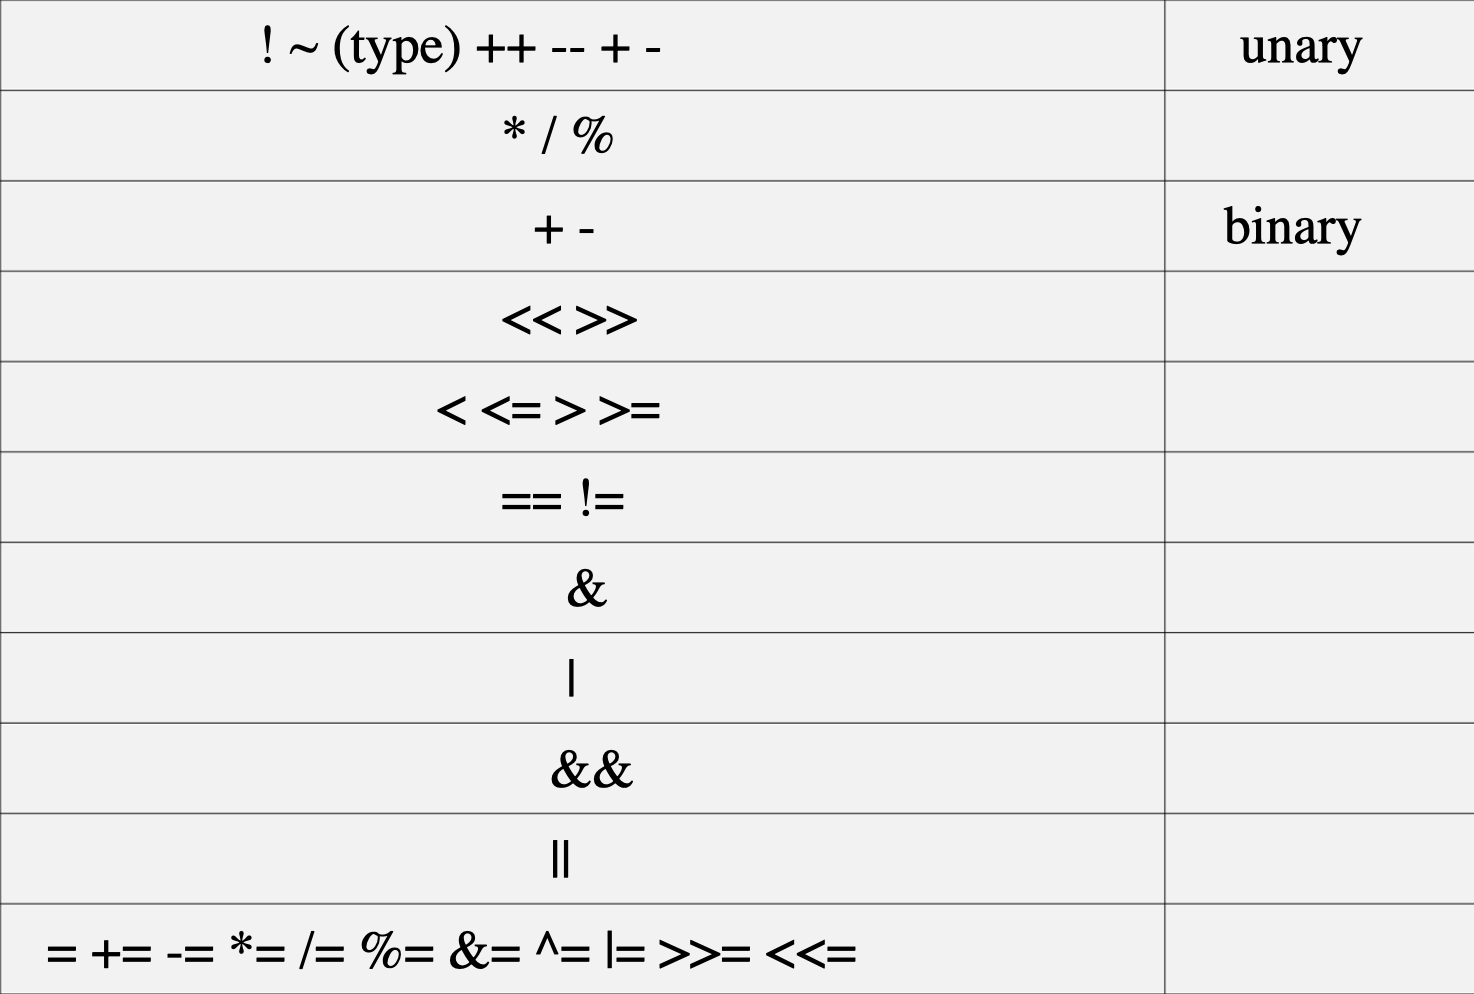
\includegraphics[width=330px]{./images/priorities.png}
\caption{Priority Table}
\end{figure}

\newpage
\section{Modules and Packages}
\label{sec:orgdd9bcbb}
\subsection{Namespace}
\label{sec:orgf9fad61}
Namespace is a space in which some names exist and the names don’t
conflict with each other; in fact \textbf{there are not} two different objects of the
same name.
\subsection{Module}
\label{sec:orgda8b2fa}

\begin{figure}[htbp]
\centering
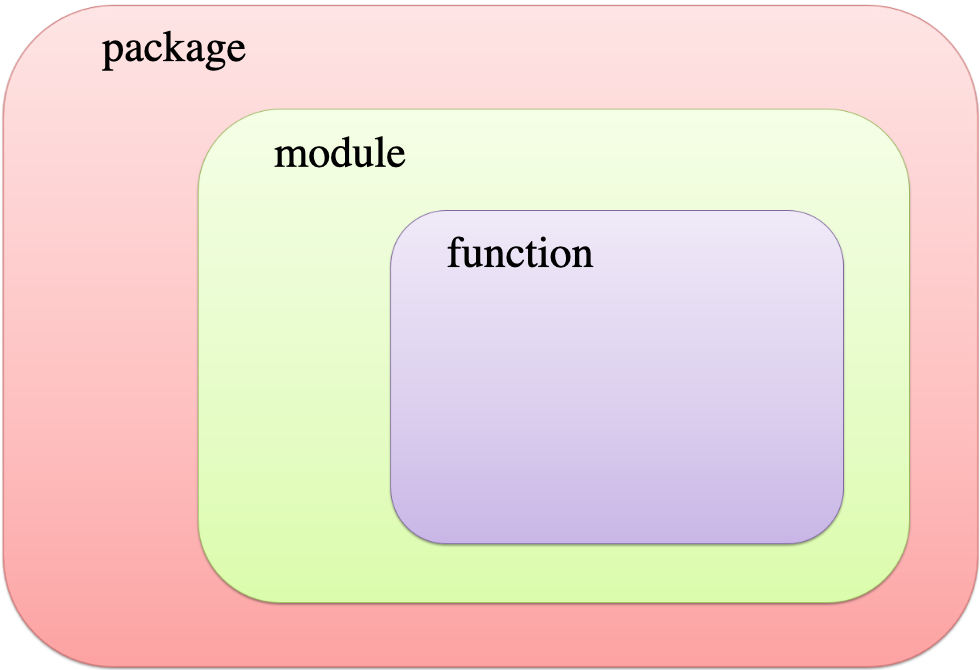
\includegraphics[width=220px]{./images/moduleHierarchy.png}
\caption{Modules and Packages Hierarchy}
\end{figure}

Python has a way to put definitions in a file and use them in a script
or in an interactive instance of the interpreter. Such a file is
called a module; a module is a \textbf{kind of container} filled with
functions. You can pack as many functions as you want into one module
and distribute it across the world;

\begin{itemize}
\item First of all, a module is identified by its name.
\item All modules, along with the built-in functions, form the
“Python standard library”. \href{https://docs.python.org/3/library/index.html}{Python Standard Library}
\item Each module consists of entities (like a book consists of
chapters). These entities can be functions, variables, constants,
classes, and objects. If you know how to access a particular module,
you can make use of any of the entities it stores.
\end{itemize}

\newpage
\subsection{Package}
\label{sec:orgb045de3}

\begin{figure}[htbp]
\centering
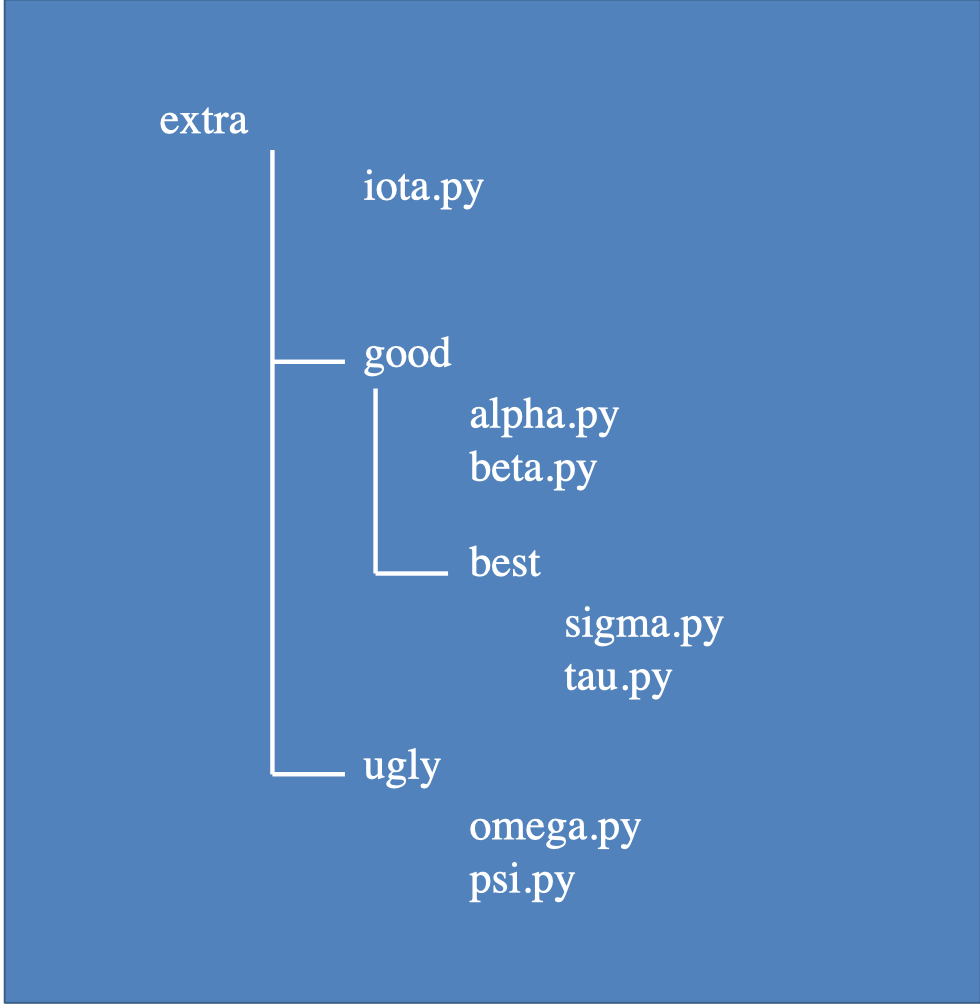
\includegraphics[width=180px]{./images/packageTree.png}
\caption{Package example tree}
\end{figure}

Making many modules may cause a little mess – sooner or
later you’ll want to group your modules exactly in the
same way as you’ve previously grouped functions, the
solution is a \textbf{package}; in the world of modules, a
package plays a similar role to a folder/directory in the
world of files.

\subsubsection{Locating package's files}
\label{sec:orgcc42ee6}
for instance according to the image above:
\begin{itemize}
\item the location of a function named FunT() from the tau package may be
described as:

\texttt{extra.good.best.tau.FunT()}

\item a function marked as below comes from the \texttt{psi} module being stored in
the \texttt{ugly} subpackage of the \texttt{extra} package.

\texttt{extra.ugly.psi.FunP()}
\end{itemize}


\subsubsection{Initialization package}
\label{sec:org354fadc}
The initialization of a module is done by an unbound code (not a part
of any function) located inside the module’s file. As a package is not
a file, this technique is useless for initializing packages. You need
to use a different trick instead – Python expects that there is a file
with a very unique name inside the package’s folder \textbf{\texttt{\_\_init\_\_.py}}.
The content of the file is executed when any of the package’s modules
is \textbf{imported}. If you don’t want any special initializations, you can
leave the file empty, but you mustn’t omit it.


\begin{itemize}
\item Note: it’s not only the “root” folder that can contain the
\texttt{\_\_init\_\_.py} file – you can put it inside any of its subfolders
(subpackages) too. It may be useful if some of the subpackages require
individual treatment and special kinds of initialization.
\end{itemize}
\subsection{Import}
\label{sec:orgb5dcd85}
\begin{description}
\item[{syntax}] \texttt{import moduleName1, moduleName2, ...}
\begin{itemize}
\item The instruction may be located anywhere in your code, but it must be
placed before the first use of any of the module’s entities.
\item The instruction imports two modules, first the one named \texttt{moduleName1} and
then the second named \texttt{moduleName2}.
\end{itemize}

\item[{syntax}] \texttt{import moduleName as alias}
\begin{itemize}
\item Aliasing causes the module to be identified under a different
name than the original. This may shorten the qualified names,
too.
\item after successful execution of an aliased import, the original
module name becomes \textbf{inaccessible} and must not be used.
\end{itemize}

\item If the module of a specified name exists and is accessible (a module
is in fact a Python source file), Python imports its contents, i.e.,
all the names defined in the module become known, but they \textbf{don’t
enter your code’s namespace.} So to use something from imported
module use have to specify it's module name to avoid conflicts
between your namespace and module namespace. Simply put:
\begin{itemize}
\item The name of the module
\item a dot;
\item The name of the entity
\end{itemize}

\item[{syntax}] \texttt{from moduleName import entity}
\begin{itemize}
\item the listed entities (and only those ones) are imported from the
indicated module;
\item the names of the imported entities \textbf{are accessible without
qualification}.
\item In this method if you assign anything to any of imported entities
or define a function with their name, you will shadow the module's
entities and from now on you don't have access to module entities
anymore!
\item \textbf{Vise versa,} if you import module's entities after some value or
functions which has the same name, the module entities will shadow
them.
\end{itemize}

\item[{syntax}] \texttt{from moduleName import *}
\begin{itemize}
\item This is like the previous condition but import all module's entities
\item \textbf{Be careful}, in this way if you don't know some module's
entities, you may cause a conflict or name shadowing
\end{itemize}

\item[{syntax}] \texttt{from moduleName import entity as alias, entity as alias, entity as alias, ...}
\begin{itemize}
\item In turn, when you use the \texttt{from module import name} variant and you
need to change the entity’s name, you make an alias for the
entity. This will cause the name to be replaced by the alias you
choose.
\item As previously, the original (unaliased) name becomes inaccessible.
\end{itemize}
\end{description}


\emph{Note: import is also a keyword (with all the
consequences of this fact).}

\subsubsection{import addressing}
\label{sec:orgeeea970}
\begin{itemize}
\item If the module is not in the same directory but the directory is a
child of current directory:
\begin{itemize}
\item \texttt{import directoryName.moduleName}
\item OR 
\begin{minted}[linenos,firstnumber=1]{python}
from sys import path
path.append("./directoryName")
import moduleName
\end{minted}
\end{itemize}
\item If the module is not in the same directory and the directory is not
a child of current directory:
\begin{itemize}
\item To be like:
\begin{minted}[linenos,firstnumber=1]{python}
from sys import path
path.append("path/to/module's/directory")
import moduleName
\end{minted}
\end{itemize}
\end{itemize}


\begin{itemize}
\item Let assume we have a package named \textbf{extra}, if we zip hole files and
directories in a zip file named \textbf{extrapack.zip} now we can \textbf{append}
this file to the \textbf{path} variable and by then we can treat the
package as it's name is \textbf{extra} not \textbf{extrapack.zip}!!! for instance
\texttt{import extra.good.best.sigma as sig} . Because python treats zip
files almost as regular file/directories
\item Remember if you import the hole module or package, every time you
want to use them you have to specify \textbf{fully qualified path} to them,
if you don't like it: 
\begin{itemize}
\item use \texttt{from ... import ...}
\item or use alias \texttt{import ... as ...}
\end{itemize}
\item We’ve used the append() method – in effect, the new path will occupy
the last element in the path list; if you don’t like the idea, you can
use insert() instead.
\item The above method works as the same also for packages

\newpage
\end{itemize}
\subsection{Creating a Module}
\label{sec:orgba7d112}
\begin{enumerate}
\item Creating a file with module name and .py extension
\item Creating a file which is named \textbf{main.py}, it contains just a line
like \texttt{import module} (of course it's not part of creating a module,
we made it to test importing the module)
\item Having this two files and executing main.py, a directory will be
created which is named \textbf{\texttt{\_\_pycache\_\_}}. This directory contains a
file most like \textbf{module.cpython-xy.pyc}
\begin{itemize}
\item The name of the file is the same as your module’s name
\item he part after the first dot says which Python implementation has
created the file (CPython here) and its version number. (xy)
\item The last part (pyc) comes from the words “Python” and “compiled”
\end{itemize}
\end{enumerate}

\subsubsection{Notes:}
\label{sec:org00816c0}
\begin{itemize}
\item When Python imports a module for the first time, it translates
its contents into a somewhat compiled shape. The file doesn’t contain
machine code – it’s internal Python semi-compiled code, ready to be
executed by Python’s interpreter. As such a file doesn’t require lots
of the checks needed for a pure source file, the execution starts
faster, and runs faster, too. Python is able to check if the module’s
source file has been modified (in this case, the \textbf{pyc} file will be
rebuilt) or not (when the \textbf{pyc} file may be run at once). As this
process is fully automatic and transparent, you don’t have to keep it
in mind.

\item When a module is imported, its content is \textbf{implicitly
executed} by Python. Be careful, so for example if you have a print()
barely in you module, it will execute!. But in fact it gives the
module the chance to initialize some of its internal aspects (e.g., it
may assign some variables with useful values). The initialization
takes place \textbf{only once}, when the first import occurs, so the
assignments done by the module aren’t repeated unnecessarily.

\begin{itemize}
\item Imagine the following context:

\begin{itemize}
\item there is a module named \texttt{mod1};
\item there is a module named \texttt{mod2} which contains the import \texttt{mod1}
instruction;
\item there is a main file containing the import \texttt{mod1} and import \texttt{mod2}
instructions.
\end{itemize}
\end{itemize}
\end{itemize}

At first glance, you may think that mod1 will be imported twice
fortunately, \textbf{only the first import occurs.} Python remembers the
imported modules and silently omits all subsequent imports.

\subsubsection{\texttt{\_\_name\_\_} variable}
\label{sec:org50b5bb1}
\begin{itemize}
\item when you run a file directly, its \texttt{\_\_name\_\_} variable is set to
\texttt{\_\_main\_\_};
\item when a file is imported as a module, its \texttt{\_\_name\_\_} variable is set to
the file’s name (excluding .py)
\end{itemize}

\subsubsection{variable deceleration}
\label{sec:org08f6e9c}
Unlike many others programming languages, Python has no means of
allowing you to hide such variables from the eyes of the module’s
users. You can only inform your users that this is your variable, that
they may read it, but that they should not modify it under any
circumstances. This is done by preceding the variable’s name with \texttt{\_}
or \texttt{\_\_}, but remember, it’s only a convention. Your module’s users may
obey it or they may not. Exp, \texttt{\_\_counter = 0}

\subsubsection{shabang}
\label{sec:org2d84c04}
\begin{description}
\item[{syntax}] \texttt{\#!/usr/bin/env python3}
\end{description}
For Unix and Unix-like OSs (including MacOS) such a line instructs the
OS how to execute the contents of the file (in other words, what
program needs to be launched to interpret the text). In some
environments (especially those connected with web servers) the absence
of that line will cause trouble;

\subsubsection{doc-string}
\label{sec:org7d18760}
\begin{description}
\item[{syntax}] \texttt{"""the module description"""}
\end{description}
a string (maybe a multiline) placed before any module instructions
(including imports) is called the doc-string, and should briefly
explain the purpose and contents of the module;

\subsection{path}
\label{sec:org7470f14}
There’s a special variable (actually a list) storing all locations
(folders/directories) that are searched in order to find a module
which has been requested by the import instruction. Python browses
these folders in the order in which they are listed in the list – if
the module cannot be found in any of these directories, the import
\textbf{fails}. Otherwise, \textbf{the first folder} containing a module with the
desired name will be taken into consideration and \emph{if any of the}
\emph{remaining folders contains a module of that name it will be}
\emph{\textbf{ignored}.} The variable is named \texttt{path}, and it’s accessible through
the module named \texttt{sys}.

\begin{itemize}
\item there is a zip file listed as one of the path’s elements – it’s not
an error. Python is able to treat zip files as ordinary folders –
this can save lots of storage.
\item the folder in which the execution starts is listed in the first
path’s element.
\end{itemize}

\subsection{dir()}
\label{sec:orge37cb12}
it is able to reveal all the names provided through a particular
module. There is one condition: the module has to have been previously
imported as a whole (i.e., using the import module instruction – from
module is not enough).  The function returns an alphabetically sorted
list containing all entities’ names available in the module identified
by a name passed to the function as an argument. 

\emph{Note: if the module’s name has been aliased, you must use the alias,
not the original name.}

\subsection{Some math functions}
\label{sec:org14084d8}
\subsubsection{pow()}
\label{sec:org5e1439a}
pow(x,y) This is a built-in function, and doesn’t have to be imported.
\subsubsection{floor() \& ceil()}
\label{sec:org5d14dbc}
floor always round to smaller number, where ceil round to bigger number

\begin{minted}[linenos,firstnumber=1]{python}

from math import ceil, floor, trunc

x = 1.4
y = 2.6
print(floor(x), floor(y))
print(floor(-x), floor(-y))
print(ceil(x), ceil(y))
print(ceil(-x), ceil(-y))
print(trunc(x), trunc(y))
print(trunc(-x), trunc(-y))

\end{minted}

\begin{verbatim}
1 2
-2 -3
2 3
-1 -2
1 2
-1 -2
\end{verbatim}

\subsubsection{random()}
\label{sec:org98dcda9}
\begin{itemize}
\item Produces a float number x coming from the range (0.0, 1.0) –in other
words: (0.0 <= x < 1.0).
\item A random number generator takes a value called a seed, treats it as
an input value, calculates a “random” number based on it.
\end{itemize}
\subsubsection{seed()}
\label{sec:org18e3845}
\begin{itemize}
\item \texttt{seed()} – sets the seed with the current time;
\item \texttt{seed(i)} – sets the seed with the integer value i.
\end{itemize}
\subsubsection{randrange()}
\label{sec:orgaf9068a}
If you want integer random values, one of the following functions
would fit better. First three one has \textbf{right-sided exclusion!} but the
last one \texttt{randint(left, right)} starts from \emph{left} and ends on \emph{right}
which also could contain \emph{right} integer

\begin{enumerate}
\item randrange(end)
\item randrange(beg,end)
\item randrange(beg, end, step)
\item randint(left, right)
\end{enumerate}


\begin{minted}[linenos,firstnumber=1]{python}
from random import randrange, randint

print(randrange(5))
print(randrange(0,5))
print(randrange(0,20,2))
print(randint(0,1))
\end{minted}

\begin{verbatim}
1
0
8
0
\end{verbatim}

\subsubsection{choice()}
\label{sec:orgb30d0e7}
\begin{description}
\item[{syntax}] \texttt{choice(sequence)}
\end{description}
Chooses a “random” element from the input sequence(list,\ldots{}) and
returns it.
\subsubsection{sample()}
\label{sec:org17fdac0}
\begin{description}
\item[{syntax}] \texttt{sample(sequence, elements\_to\_chose=1)}
\end{description}
Chooses some of the input elements(default in one), returning a list with the
choice. The elements in the sample are placed in random order. Note:
the \texttt{elements\_to\_chose} must not be greater than the length of the input
sequence.


\begin{minted}[linenos,firstnumber=1]{python}
from random import sample
lst = list(range(0, 10))
print(sample(lst, 5))
\end{minted}

\begin{verbatim}
[9, 5, 2, 7, 1]
\end{verbatim}


\newpage

\subsection{Some platform functions}
\label{sec:org69fa4c9}
\subsubsection{platform()}
\label{sec:org01ce961}
\begin{description}
\item[{syntax}] 
\end{description}
\begin{minted}[linenos,firstnumber=1]{python}
from platform import platform
platform(aliased=False, terse=False)
\end{minted}

\begin{itemize}
\item aliased→ when set to True (or any non-zero value) it may cause the
function to present the alternative underlying layer names instead
of the common ones;
\item terse→ when set to True (or any non-zero value) it may convince
the function to present a briefer form of the result (if possible)
\end{itemize}

\subsubsection{machine()}
\label{sec:org2eae2a8}
\begin{description}
\item[{syntax}] 
\end{description}
\begin{minted}[linenos,firstnumber=1]{python}
from platform import machine
print(machine())
\end{minted}

\begin{verbatim}
x86_64
\end{verbatim}

\begin{itemize}
\item Sometimes, you may just want to know the generic name of the
processor which runs your OS together with Python and your code – a
function named machine() will tell you that. As previously, the
function returns a string.
\end{itemize}

\subsubsection{processor()}
\label{sec:org7c32bb8}
\begin{description}
\item[{syntax}] 
\end{description}
\begin{minted}[linenos,firstnumber=1]{python}
from platform import processor
print(processor())
\end{minted}

\begin{verbatim}
i386
\end{verbatim}

\begin{itemize}
\item The processor() function returns a string filled with the real
processor name (if possible)
\end{itemize}

\subsubsection{system()}
\label{sec:org1801898}
\begin{description}
\item[{syntax}] 
\end{description}
\begin{minted}[linenos,firstnumber=1]{python}
from platform import system
print(system())
\end{minted}

\begin{verbatim}
Darwin
\end{verbatim}

\begin{itemize}
\item A function named system() returns the generic OS name as a string
\end{itemize}

\subsubsection{version()}
\label{sec:org75907a5}
\begin{description}
\item[{syntax}] 
\end{description}
\begin{minted}[linenos,firstnumber=1]{python}
from platform import version
print(version())
\end{minted}

\begin{verbatim}
Darwin Kernel Version 18.2.0: Mon Nov 12 20:24:46 PST 2018; root:xnu-4903.231.4~2/RELEASE_X86_64
\end{verbatim}

\begin{itemize}
\item The OS version is provided as a string by the version() function
\end{itemize}

\subsubsection{python info}
\label{sec:org7559285}
\begin{description}
\item[{syntax}] 
\end{description}
\begin{minted}[linenos,firstnumber=1]{python}
from platform import python_implementation, python_version_tuple
print(python_implementation())
print(python_version_tuple())
\end{minted}

\begin{verbatim}
CPython
('3', '7', '1')
\end{verbatim}

\begin{itemize}
\item \texttt{python\_implementation()} → returns a string denoting the Python
implementation (expect 'CPython' here, unless you decide to use any
non-canonical Python branch)
\item \texttt{python\_version\_tuple()} → returns a three-element tuple filled with:
\begin{itemize}
\item the major part of Python’s version;
\item the minor part;
\item the patch level number
\item for exp:  ('3', '7', '0')
\end{itemize}
\end{itemize}

\section{Error and Exception}
\label{sec:org90d47f7}
\subsection{Raising an exception}
\label{sec:org99185c1}
Each time your code tries to do something
wrong/foolish/irresponsible/crazy/unenforceable, Python does two
things:

\begin{itemize}
\item it stops your program;
\item it creates a special kind of data, called an exception.
\end{itemize}

Both of these activities are called raising an exception.We can say
that Python always raises an exception (or that an exception has been
raised) when it has no idea what do to with your code.

\subsection{try - except}
\label{sec:orga91366f}
\begin{enumerate}
\item the \texttt{try} keyword begins a block of the code which may or may not be
performing correctly;
\item next, Python tries to perform the risky action; if it fails, an
exception is raised and Python starts to look for a solution;
\item \texttt{except} keyword starts a piece of code which will be executed if
anything inside the try block goes wrong – if an exception is
raised inside a previous try block, it will fail here, so the code
located after the except keyword should provide an adequate
reaction to the raised exception;
\item \textbf{returning} to the previous nesting level ends the try-except
section.
\end{enumerate}


Sample code:
\begin{minted}[linenos,firstnumber=1]{python}
a = 1
b = 0

try:
    print("START")
    print(a / b)
except:
    print('It cannot be done!')

print('THE END')

\end{minted}

\begin{verbatim}
START
It cannot be done!
THE END
\end{verbatim}

Note: Code block inside the \texttt{try} will execute until first error and
after that python will immediately jumps out of the block and into the
first instruction located after the except: keyword; this means that
\textbf{some} of the instructions from the block may be silently omitted.

\subsubsection{try - multiple exceptions}
\label{sec:orgf45905d}
\begin{itemize}
\item syntax
\begin{itemize}
\item if an unnamed except branch exists (one without an exception
name), it has to be specified as the last.
\item In case you do not have any general exception(unnamed except), if
none of the specified named except branches matches the raised
exception, the exception remains unhandled.
\end{itemize}
\end{itemize}

\begin{minted}[linenos,firstnumber=1]{python}
try:
    .
    .
except exc1:
    .
    .
except exc2:
    .
    .
except:
    .
    .
\end{minted}

\begin{minted}[linenos,firstnumber=1]{python}
try:
    .
    .
except (exc1, exc2)
    .
    .
except:
    .
    .
\end{minted}

\begin{itemize}
\item Sample code
\end{itemize}
\begin{minted}[linenos,firstnumber=1]{python}
try:
    x = 0
    y = 1 / x
    print(y)
except ZeroDivisionError:
    print('Cannot divide by zero sorry')
except ValueError:
    print('You have to enter an integer value')
except:
    print('Oh, dear')

print('THE END')
\end{minted}

\begin{verbatim}
Cannot divide by zero sorry
THE END
\end{verbatim}



\newpage
\subsubsection{finally}
\label{sec:org70cd0ab}
Code in a finally statement even runs if an uncaught exception occurs
in one of the preceding blocks.

\begin{minted}[linenos,firstnumber=1]{python}
try:
    print(1)
    print(10 / 0)
except ZeroDivisionError:
    print('unknown_var')
finally:
    print("This is executed last")
\end{minted}

\begin{verbatim}
1
unknown_var
This is executed last
\end{verbatim}

\subsection{Anatomy of exceptions}
\label{sec:org6d4dcbb}

\begin{figure}[htbp]
\centering
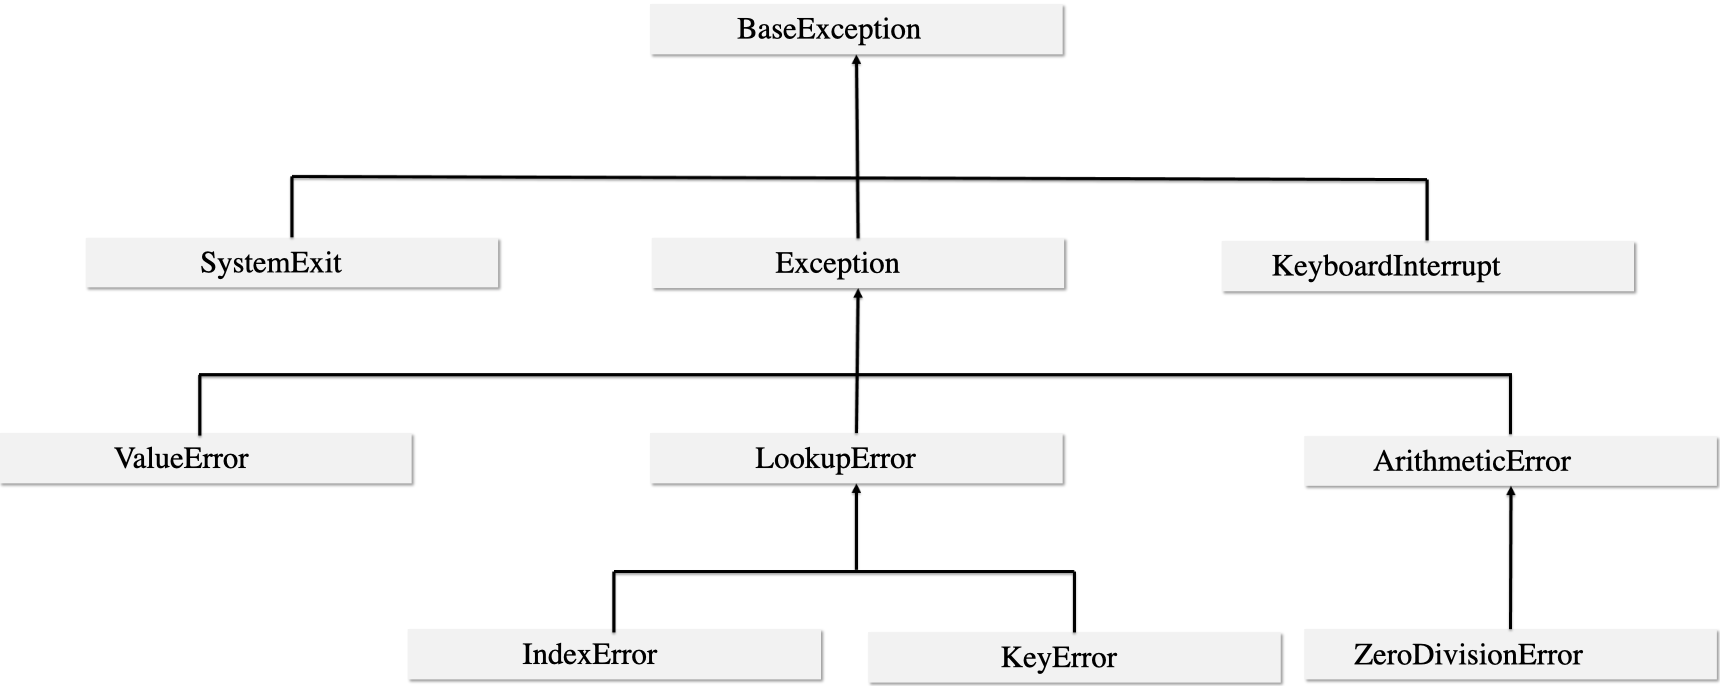
\includegraphics[width=320px]{./images/exceptions.png}
\caption{Exception tree}
\end{figure}

Some of the built-in exceptions are more general (they include other
exceptions) while others are completely concrete (they represent
themselves only). We can say that the closer to the root an exception
is located, the more general (abstract) it is. In turn, the exceptions
located at the branches’ ends (we can call them leaves) are concrete.

\begin{itemize}
\item \textbf{The order of the branches matters!}
\item don’t put more general exceptions before more concrete ones;
\item each raised exception falls into the first matching branch;
\item the matching branch doesn’t have to specify the same exception
exactly – it’s enough that the exception is more general (more
abstract) than the raised one.
\end{itemize}

\subsection{Some useful exceptions}
\label{sec:org069a900}
\subsubsection{BaseException ← Exception ← ArithmeticError}
\label{sec:org2ac25f6}
an abstract exception including all exceptions caused by arithmetic
operations like zero division or an argument’s invalid domain

\subsubsection{BaseException ← Exception ← AssertionError}
\label{sec:org52a8022}
a concrete exception raised by the assert instruction when its
argument evaluates to \textbf{False, None, zero, or an empty string}

\begin{minted}[linenos,firstnumber=1]{python}
from math import tan,radians
angle = int(input('Enter integral angle in degrees: '))
# we must be sure that angle != 90 + k*180
assert angle % 180 != 90
print(tan(radians(angle)))
\end{minted}

\subsubsection{BaseException}
\label{sec:org9b7fc79}
the most general (abstract) of all Python exceptions – all other
exceptions are included in this one; it can be said that the following
two except branches are equivalent:

\texttt{except:}

\texttt{except BaseException:}

\subsubsection{BaseException ← Exception ← LookupError ← IndexError}
\label{sec:org0e3ebfa}
a concrete exception raised when you try to access a non-existent
sequence’s element (e.g., a list’s)

\begin{minted}[linenos,firstnumber=1]{python}
# the code shows an extravagant way of leaving the loop
list = [1,2,3,4,5]
ix = 0
doit = True
while doit:
    try:
	print(list[ix])
	ix += 1
    except IndexError:
	doit = False
print('Done')
\end{minted}

\subsubsection{BaseException ← Exception ← LookupError}
\label{sec:org4bd7724}
an abstract exception including all exceptions caused by errors
resulting from invalid references to different collections (lists,
dictionaries, tuples, etc.)

\subsubsection{BaseException ← KeyboardInterrupt}
\label{sec:orgd7be734}
a concrete exception raised when the user uses a keyboard shortcut
designed to terminate a program’s execution (Ctrl-C in most OSs); if
handling this exception doesn’t lead to program termination, the
program continues its execution. Note: this exception is not derived
from the Exception class.

\begin{minted}[linenos,firstnumber=1]{python}
# this code cannot be terminated by pressing Ctrl-C
from time import sleep
seconds = 0
while True:
    try:
	print(seconds)
	seconds += 1
	sleep(1)
    except KeyboardInterrupt:
	print("Don't do that!")
\end{minted}

\subsubsection{BaseException ← Exception ← MemoryError}
\label{sec:org815db98}
a concrete exception raised when an operation cannot be completed due
to a lack of free memory

\begin{minted}[linenos,firstnumber=1]{python}
# this code causes the MemoryError exception
# warning: executing this code may be crucial for your OS
# don't run it in production environments!

string = 'x'
try:
    while True:
	string = string + string
	print(len(string))
except MemoryError:
    print('This is not funny!')
\end{minted}

\subsubsection{BaseException ← Exception ← ArithmeticError ← OverflowError}
\label{sec:org8101f7e}
a concrete exception raised when an operation produces a number too
big to be successfully stored

\begin{minted}[linenos,firstnumber=1]{python}
# the code prints subsequent values of exp(k), k = 1,2,4,8,16,…
from math import exp
ex = 1
try:
    while True:
	print(exp(ex))
	ex *= 2
except OverflowError:
    print('Number is too big.')

\end{minted}

\subsubsection{BaseException ← Exception ← StandardError ← ImportError}
\label{sec:orga0036e8}
a concrete exception raised when an import operation fails

\begin{minted}[linenos,firstnumber=1]{python}
# one of this imports will fail - which one?
try:
    import math
    import time
    import abracadabra
except:
    print('One of your imports has failed. ')
\end{minted}

\subsubsection{BaseException ← Exception ← LookupError ← KeyError}
\label{sec:org9c849f3}
a concrete exception raised when you try to access a non-existent
collection’s element (e.g., a dictionary’s)

\begin{minted}[linenos,firstnumber=1]{python}
# how to abuse the dictionary and how to deal with it
dict = { 'a' : 'b', 'b' : 'c', 'c' : 'd' }
ch = 'a'
try:
    while True:
	ch = dict[ch]
	print(ch)
except KeyError:
    print('No such key:', ch)

\end{minted}

\begin{verbatim}
b
c
d
No such key: d
\end{verbatim}

\subsection{raise}
\label{sec:org762c25b}
The raise instruction raises the specified exception named exc as if
it was raised in a normal
\begin{itemize}
\item \textbf{simulate} raising actual exceptions (e.g., to test your handling
strategy)
\item \textbf{partially handle} an exception and make another part of the code
responsible for completing the handling (separation of concerns).
\item The \texttt{raise} instruction may also be utilized without any exception
name.
\begin{itemize}
\item this kind of raise instruction may be used inside the except
branch \textbf{only};
\item using it in any other context \textbf{causes an error}.
\item The instruction will \textbf{immediately re-raise the same exception as
currently handled.}
\end{itemize}
\begin{minted}[linenos,firstnumber=1]{python}
def badfun(n):
    try:
	return n/0
    except:
	print('I did it again!')
	raise

try:
    badfun(0)
except ArithmeticError:
    print('I see!')
print('THE END')
\end{minted}

\begin{verbatim}
I did it again!
I see!
THE END
\end{verbatim}

\item Exceptions can be raised with arguments that give detail about them.
\end{itemize}

\begin{minted}[linenos,firstnumber=1]{python}
name = "123"
raise NameError("Invalid name!")
\end{minted}

\subsection{assert}
\label{sec:orgce7f38e}
How does it work?
\begin{itemize}
\item It evaluates the expression;
\item if the expression evaluates to True, or a non-zero numerical value,
or a non-empty string, or any other value different than None and
False, it won’t do anything else;
\item otherwise, it automatically and immediately raises an exception
named AssertionError (in this case, we say that the assertion has
failed)
\end{itemize}

How it can be used?
\begin{itemize}
\item you may want to put it into your code where you want to be
absolutely safe from evidently wrong data, and where you aren’t
absolutely sure that the data has been carefully examined before
(e.g., inside a function used by someone else)
\item raising an \texttt{AssertionError} exception secures your code from producing
invalid results, and clearly shows the nature of the failure;
\item assertions don’t supersede exceptions or validate the data – they
are their supplements.
\item It's also very good to use it for documentation of your code
\end{itemize}

\begin{minted}[linenos,firstnumber=1]{python}
import math
x = float(input())
assert x>=0.0
x = math.sqrt(x)
print(x)
\end{minted}

\begin{itemize}
\item The assert can take a second argument that is passed to the
AssertionError raised if the assertion fails.
\end{itemize}

\begin{minted}[linenos,firstnumber=1]{python}
temp = -10
assert (temp >= 0), "Colder than absolute zero!"
\end{minted}

\subsection{else}
\label{sec:orgf6677d5}
\textbf{A code labelled in this way is executed when (and only when) no}
\textbf{exception has been raised inside the \texttt{try} part}.  We can say that
exactly one branch can be executed after \texttt{try:} either the one
beginning with \texttt{except} (don’t forget that there can be more than one
branch of this kind) or the one starting with \texttt{else}. Note that the
else branch has to be located after the last except branch.

\begin{minted}[linenos,firstnumber=1]{python}
def reciprocal(n):
	try:
		n = 1 / n
	except ZeroDivisionError:
		print("Division failed")
		return None
	else:
		print("Everything went fine")
		return n


print(reciprocal(2))
print(reciprocal(0))
\end{minted}

\subsection{finally}
\label{sec:orgb20e710}
The \texttt{try-except} block can be extended in one more way – by adding a
part headed by the \texttt{finally} keyword (it must be the last branch of
the code designed to handle exceptions). Note that these two variants
(\texttt{else} and \texttt{finally}) aren’t dependent in any way, and they can
coexist or occur independently. The finally block is always executed
(it finalizes the try-except block execution, hence its name), no
matter what happened earlier, even when raising an exception, no
matter whether this has been handled or not.

\begin{minted}[linenos,firstnumber=1]{python}
def reciprocal(n):
	try:
		n = 1 / n
	except ZeroDivisionError:
		print("Division failed")
		n = None
	else:
		print("Everything went fine")
	finally:
		print("It's time to say good bye")
		return n

print(reciprocal(2))
print(reciprocal(0))
\end{minted}

\subsection{Exception Object}
\label{sec:org57473d3}
You probably won’t be surprised to learn that exceptions are
classes. Furthermore, when an exception is raised, an object of the
class is instantiated, and goes through all levels of program
execution, looking for the except branch that is prepared to deal with
it.  Such an object carries some useful information which can help you
to precisely identify all aspects of the pending situation. To achieve
that goal, Python offers a special variant of the exception clause

In the code below you can see, the except statement is extended, and
contains an additional phrase starting with the as keyword, followed
by an identifier. The identifier is designed to catch the exception
object so you can analyze its nature and draw proper conclusions. Note
that the identifier’s scope covers its \texttt{except} branch, and doesn’t go
any further.

\begin{minted}[linenos,firstnumber=1]{python}
try:
	i = int("hello!")
except Exception as e:
	print(e)
	print(e.__str__())

\end{minted}

\subsection{Extending Exceptions}
\label{sec:org7bf1461}
The exceptions hierarchy is neither closed nor finished, and you can
always extend it if you want or need to create your own world
populated with your own exceptions. It may be useful when you create a
complex module which detects errors and raises exceptions, and you
want the exceptions to be easily distinguishable from any others
brought by Python.

This is done by defining your own, new exceptions as subclasses
derived from predefined ones.  Note that if you want to create an
exception which will be utilized as a specialized case of any built-in
exception, derive it from just this one. If you want to build your own
hierarchy, and don’t want it to be closely connected to Python’s
exception tree, derive it from any of the top exception classes, like
Exception.

In the code sample below we’ve defined our own exception, named
\textbf{MyZeroDivisionError}, derived from the built-in
\textbf{ZeroDivisionError}. As you can see, we’ve decided not to add any new
components to the class. In effect, an exception of this class can be
– depending of the desired point of view – treated like a plain
ZeroDivisionError, or considered separately.  The \textbf{doTheDivision()}
function raises either a \textbf{MyZeroDivisionError} or \textbf{ZeroDivisionError}
exception, depending on the argument’s value. The function is invoked
four times in total, while the first two invocations are handled using
only one except branch (the more general one) and the last two ones
with two different branches, able to distinguish the exceptions (don’t
forget: the order of the branches makes a fundamental difference!)

\begin{minted}[linenos,firstnumber=1]{python}
class MyZeroDivisionError(ZeroDivisionError):
	pass

def doTheDivision(mine):
	if mine:
		raise MyZeroDivisionError("worse news")
	else:		
		raise ZeroDivisionError("bad news")

for mode in [False, True]:
	try:
		doTheDivision(mode)
	except ZeroDivisionError:
		print('Division by zero')


for mode in [False, True]:
	try:
		doTheDivision(mode)
	except MyZeroDivisionError:
		print('My division by zero')
	except ZeroDivisionError:
		print('Original division by zero')		
\end{minted}

\begin{verbatim}
Division by zero
Division by zero
Original division by zero
My division by zero
\end{verbatim}

\newpage
\subsection{Extending Exceptions Example}
\label{sec:org369675d}
Here we've provided a good and yet simple example to help you
understand extending exception from the scratch!

\begin{minted}[linenos,firstnumber=1]{python}
class PizzaError(Exception):
    def __init__(self, pizza, message):
	Exception.__init__(self,message)
	self.pizza = pizza

class TooMuchCheeseError(PizzaError):
    def __init__(self, pizza, cheese, message):
	PizzaError.__init__(self,pizza,message)
	self.cheese = cheese

def makePizza(pizza,cheese):
	if pizza not in ['margherita', 'capricciosa', 'calzone']:
		raise PizzaError(pizza,"no such pizza in menu")
	if cheese > 100:
		raise TooMuchCheeseError(pizza, cheese, "too much cheese")
	print("Pizza ready!")

for (pz,ch) in [('calzone',0),('margherita',110),('mafia',20)]:
	try:
		makePizza(pz,ch)
	except TooMuchCheeseError as tmce:
		print(tmce, ':', tmce.cheese)
	except PizzaError as pe:
		print(pe, ':', pe.pizza)
\end{minted}

\begin{verbatim}
Pizza ready!
too much cheese : 110
no such pizza in menu : mafia
\end{verbatim}

\newpage

\section{Strings}
\label{sec:org978b6de}
\subsection{Terminology}
\label{sec:orgfbbca46}
\begin{itemize}
\item Computers store characters as numbers. Every character used by a
computer corresponds to a unique number, and vice versa.
\item The word “internationalization” is commonly shortened to I18N → Why?
Look carefully – there is an I at the front of the word, next there
are 18 different letters, and an N at the end.
\item A classic form of ASCII code uses eight bits for each sign. Eight
bits mean 256 different characters. The first 128 are used for the
standard Latin alphabet (both upper-case and lower-case characters).
\item A \textbf{code point} is a number which makes a character. For example, 32
is a code point which makes a space in ASCII encoding. We can say
that standard ASCII code consists of 128 code points.
\item A \textbf{code page} is a standard for using the upper 128 code points to
store specific national characters. This means that the one and same
code point can make different characters when used in different code
pages.
\item In consequence, to determine the meaning of a specific code point,
you have to know the target code page.
\item \textbf{Unicode} assigns unique (unambiguous) characters (letters, hyphens,
ideograms, etc.) to more than a million code points.
\item The first 128 Unicode code points are identical to ASCII, and the
first 256 Unicode code points are identical to the ISO/IEC 8859-1
code page (a code page designed for western European languages).
\item \textbf{UCS-4 uses 32 bits} (four bytes) to store each character, and the
code is just the Unicode code points’ unique number. A file
containing UCS-4 encoded text may start with a BOM (byte order
mark), an unprintable combination of bits announcing the nature of
the file’s contents. Some utilities may require it. As you can see,
UCS-4 is a rather wasteful standard – it increases a text’s size by
four times compared to standard ASCII.
\item \textbf{UTF-8} The name is derived from Unicode Transformation Format.The
concept is very smart. UTF-8 uses as many bits for each of the code
points as it really needs to represent them. For example all Latin
characters (and all standard ASCII characters) occupy eight bits;
and non-Latin characters occupy 16 bits and non-Latin characters
occupy 16 bits;
\item \textbf{Python3 is completely I18Ned} because it fully supports Unicode and
UTF-8:
\begin{itemize}
\item you can use Unicode/UTF-8 encoded characters to name variables and
other entities;
\item you can use them during all input and output.
\end{itemize}
\item Don’t forget that a backslash ($\backslash$) used as an escape character is \textbf{not included} 
in the string’s total length.
\item Python’s strings are \textbf{immutable sequences}. so:
\begin{itemize}
\item \texttt{del text[0]} does not work. The only thing you can do with \texttt{del} and a string is to remove the string as a whole.
\item Obviously you can't use \texttt{text.append('g')}, as the same for \texttt{insert()}
\item Don’t think that a string’s immutability limits your ability to
operate with strings. The only consequence is that you have to
remember about it, and implement your code in a slightly different
way – look at the example:
\end{itemize}
\end{itemize}

\begin{minted}[linenos,firstnumber=1]{python}
text = "fgakjgkasdjgaga"
text = "A" + text
text = text + "Z"
print(text)
\end{minted}

\begin{verbatim}
AfgakjgkasdjgagaZ
\end{verbatim}

\subsection{Multiline string}
\label{sec:orgce283a7}
The string has to start with three apostrophes, not one. The same
tripled apostrophe is used to terminate it. The number of text lines
put inside such a string is arbitrary. The multiline strings can be
delimited by triple quotes, too. The code below return 15 as result,
because \texttt{\textbackslash{}n} will count in length in python

\begin{minted}[linenos,firstnumber=1]{python}

MultiLine = '''Line #1
Line #2'''

print('The string length is: ', end='')
print(len(MultiLine))

\end{minted}

\begin{verbatim}
The string length is: 15
\end{verbatim}

\subsection{comparing}
\label{sec:org0bdb181}
\begin{itemize}
\item The final relation between strings is determined by comparing the
first different character in both strings (keep ASCII/UNICODE code
points in mind at all times)
\item When you compare two strings of different lengths and \textbf{the shorter
one is identical to the longer one’s beginning}, the longer string is
considered greater.
\item Even if a string contains digits only, it’s still not a number. It’s
interpreted as-is, like any other regular string, and its
(potential) numerical aspect is not taken into consideration in any
way.
\item Comparing strings against numbers is generally a bad idea. The only
comparisons you can perform with impunity are these symbolized by
the \texttt{= and !} operators. The former always gives False, while the
latter always produces True. Using any of the remaining comparison
operators will raise a TypeError exception.
\end{itemize}

\newpage
\subsection{Operations}
\label{sec:org35cb361}
\subsubsection{concatenated}
\label{sec:orgc658bb8}
The + operator used against two or more strings produces a new string
containing all the characters from its arguments (note: the order
matters – this overloaded +, in contrast to its numerical version,
is not commutative)

\subsubsection{Replicated}
\label{sec:orgef3c468}
the * operator needs a string and a number as arguments; in this case,
the order doesn’t matter – you can put the number before the string,
or vice versa, the result will be the same – a new string created by
the nth replication of the argument’s string.

\subsubsection{ord()}
\label{sec:org2384b9c}
If you want to know a specific character’s ASCII/UNICODE code point
value, you can use a function named ord() (as in ordinal).

\subsubsection{chr()}
\label{sec:orgd7f8145}
If you know the code point (number) and want to get the corresponding
character, you can use a function named chr().

\subsubsection{slice}
\label{sec:org8f1bb97}
Moreover, everything you know about slices is still usable. 

\begin{minted}[linenos,firstnumber=1]{python}
alpha = "abdefg"
print(alpha[1:3])
print(alpha[3:])
print(alpha[:3])
print(alpha[3:-2])
print(alpha[-3:4])
print(alpha[::2])
print(alpha[1::2])
\end{minted}

\begin{verbatim}
bd
efg
abd
e
e
adf
beg
\end{verbatim}

\subsubsection{min()}
\label{sec:org41f3abe}
The function finds the minimum element of the sequence passed as an
argument. There is one condition – the sequence (string, list, it
doesn’t matter) cannot be empty, or else you’ll get a ValueError
exception. According to ASCII table upper case alphabet less than
normal case of an alphabet

\begin{minted}[linenos,firstnumber=1]{python}
t = 'The Knights Who Say Ni'
print('[' + min(t) + ']')
t = [ 0, 2, 3 ]
print(min(t))
\end{minted}

\begin{verbatim}
[K]
0
\end{verbatim}
\subsubsection{index()}
\label{sec:org5f5ccc7}
The \texttt{index()} method (it’s a method, not a function) searches the
sequence from the beginning, in order to find the first element of the
value specified in its argument. Note that the element searched for must
occur in the sequence – its absence will cause a \texttt{ValueError} exception.
exp: \texttt{print('sdfaksdgagalrkg'.index(k))}
\subsubsection{list()}
\label{sec:orga46de23}
The list() function takes its argument (a string) and creates a new
list containing all the string’s characters, one per list
element. Note that t’s not strictly a string function – list() is able
to create a new list from many other entities (e.g., from tuples and
dictionaries).

\begin{minted}[linenos,firstnumber=1]{python}
print(list('salam'))
\end{minted}

\begin{verbatim}
['s', 'a', 'l', 'a', 'm']
\end{verbatim}
\subsubsection{count()}
\label{sec:orgc1de9af}
The count() method counts all occurrences of the element inside the
sequence. The absence of such elements doesn’t cause any problems.
\subsubsection{sorted() vs sort()}
\label{sec:orgd3027dc}
\begin{itemize}
\item \textbf{sorted()} The function takes one argument (a list) and returns a new list,
filled with the sorted argument’s elements.
\item \textbf{sort()} affects the list itself – no new list is created. Ordering
is performed in situ by the method named sort() so it's not useful for strings
\end{itemize}

\newpage
\subsection{String methods}
\label{sec:org864555a}
Note: methods don’t have to be invoked from within variables
only. They can be invoked directly from within string literals. We’re
going to use that convention regularly

\subsubsection{capitalize()}
\label{sec:orgc13bd42}
\begin{itemize}
\item if the first character inside the string is a letter (note: the
first character is an element with an index equal to 0, not just the
first visible character), it will be converted to upper-case;
\item all remaining letters from the string will be converted to
lower-case.
\item the original string (from which the method is invoked) is not
changed in any way
\item the modified (capitalized in this case) string is returned as a
result – if you don’t use it in any way (assign it to a variable, or
pass it to a function/method) it will disappear without a trace.
\end{itemize}

\begin{minted}[linenos,firstnumber=1]{python}
print('Alpha'.capitalize())
print('ALPHA'.capitalize())
print(' Alpha'.capitalize())
print('123'.capitalize())
print("άλφα".capitalize())
\end{minted}

\begin{verbatim}
Alpha
Alpha
 alpha
123
Άλφα
\end{verbatim}

\subsubsection{center()}
\label{sec:orgbcc48e5}
\begin{itemize}
\item The one-parameter variant of the center() method makes a copy of the
original string, trying to center it inside a field of a specified
width. The centering is actually done by adding some spaces before
and after the string. Don’t expect this method to demonstrate any
sophisticated skills. It’s rather simple. The example uses brackets
to clearly show you where the centered string actually begins and
terminates
\item The two-parameter variant of center() makes use of the character
from the second argument, instead of a space
\end{itemize}

\begin{minted}[linenos,firstnumber=1]{python}
print('['+'alpha'.center(1)+']')
print('['+'alpha'.center(30)+']')
print('['+'alpha'.center(10)+']')
print('['+'alpha'.center(10, '*')+']')
\end{minted}

\begin{verbatim}
[alpha]
[            alpha             ]
[  alpha   ]
[**alpha***]
\end{verbatim}

\subsubsection{endswith()}
\label{sec:orgc7898e7}
The endswith() method checks if the given string ends with the
specified argument and returns True or False, depending of the check
result.

\begin{minted}[linenos,firstnumber=1]{python}
t = 'zeta'
print(t.endswith('a'))
print(t.endswith('A'))
print(t.endswith('et'))
\end{minted}

\begin{verbatim}
True
False
False
\end{verbatim}

\subsubsection{startswitch()}
\label{sec:orga5f3221}
The startswith() method is a mirror reflection of endswith() ­– it
checks if a given string starts with the specified substring.
\subsubsection{find()}
\label{sec:org8bd25ab}
\begin{itemize}
\item The find() method is similar to index(), which you already know (it
looks for a substring), but: it’s safer – it doesn’t generate an
error for an argument containing a non-existent substring (it
returns -1 then) \textbf{it works with strings only} – don’t try to apply
it to any other sequence.
\item If you want to perform the find, not from the string’s beginning,
but from any position, you can use a two-parameter variant of the
find() method → The second argument specifies the index at which the
search will be started (it doesn’t have to fit inside the string).
\item There is also a three-parameter mutation of the find() method – the
third argument points to the first index which won’t be taken into
consideration during the search (it’s actually the upper limit of
the search) → The second argument specifies the index at which the
search will be started (it doesn’t have to fit inside the string)
\end{itemize}

\textbf{don’t use find() if you only want to check if a single character
occurs within a string – the in operator will be significantly faster.}

\begin{minted}[linenos,firstnumber=1]{python}
# if it finds the string, it will return the first index where the string appears 

print("--------------------")
t = 'theta'
print(t.find('eta'))
print(t.find('ta'))
print(t.find('the'))
print(t.find('tlhe'))

print("--------------------")

print('kappa'.find('a',2))
print('kappa'.find('a', 2, 4))
print('kappa'.find('a',8))

print("--------------------")

txt = ''' A variation of the ordinary lorem ipsum text has been used in
typesetting since the 1960s or earlier, when it was popularized by
advertisements for Letraset transfer sheets. It was introduced to the
Information Age in the mid-1980s by Aldus Corporation, which employed
it in graphics and word-processing templates for its desktop
publishing program PageMaker.'''

fnd = txt.find('the')
while fnd != -1:
    print(fnd, end="' ")
    fnd = txt.find('the', fnd+1)
\end{minted}

\begin{verbatim}
--------------------
2
3
0
-1
--------------------
4
-1
-1
--------------------
16' 81' 196' 219' 
\end{verbatim}

\subsubsection{rfind()}
\label{sec:orgd73860d}
The one-, two-, and three-parameter methods named rfind() do nearly
the same things as their counterparts (the ones devoid of the r
prefix), but start their searches from the end of the string, not the
beginning (hence the prefix r, for right).

\begin{minted}[linenos,firstnumber=1]{python}
t = 'tau tau tau'
tIndex = dict()

for i in range(len(t)):
    tIndex[i] = t[i]


for key in tIndex:
    print(key, ":", tIndex[key])


print("--------------------")
print(t.rfind('ta'))
print(t.rfind('ta',9))
print(t.rfind('ta',3,9))
\end{minted}

\begin{verbatim}
0 : t
1 : a
2 : u
3 :  
4 : t
5 : a
6 : u
7 :  
8 : t
9 : a
10 : u
--------------------
8
-1
4
\end{verbatim}

\subsubsection{isalnum()}
\label{sec:org7944cd8}
The parameterless method named isalnum() checks if the string contains
only digits or alphabetical characters (letters), and returns
True/False according to the result →

Note: any string element that is not a digit or a letter causes the
method to return False. An empty string does, too.

\begin{minted}[linenos,firstnumber=1]{python}
print('is all'.isalnum())
print('10E4'.isalnum())
print(''.isalnum())
\end{minted}

\begin{verbatim}
False
True
False
\end{verbatim}

\subsubsection{isalpha()}
\label{sec:org6d35e8e}
The isalpha() method is more specialized – it’s interested in letters
only

\subsubsection{isdigit()}
\label{sec:org7698e55}
In turn, the isdigit() method looks at digits only – anything else
produces False as the result.

\subsubsection{islower()}
\label{sec:org3b280a9}
The islower() method is a fussy variant of isalpha() – it accepts
lower-case letters only.

\subsubsection{isupper()}
\label{sec:org236f12a}
The isupper() is the upper-case version of islower() – it concentrates
on upper-case letters only.

\subsubsection{isspace()}
\label{sec:orgf582f54}
The isspace() method identifies whitespaces only – it disregards any
other character (the result is False then). Note that \texttt{\textbackslash{}n} is a whitespace
\subsubsection{join()}
\label{sec:org37a322e}
The join() method is rather complicated, so let us guide you step by
step thorough it:
\begin{itemize}
\item as its name suggests, the method performs a join – it expects one
argument as a list; it must be assured that all the list’s elements
are strings – the method will raise a TypeError exception otherwise;
\item all the list’s elements will be joined into one string but \ldots{}
\item the string from which the method has been invoked is used as a
separator, put among the strings; it can be empty or whitespace also
or arbitrary long
\item the newly created string is returned as a result.
\end{itemize}

\begin{minted}[linenos,firstnumber=1]{python}
print(','.join(['omicron','pi','rho']))
print(' '.join(['omicron','pi','rho']))
\end{minted}

\begin{verbatim}
omicron,pi,rho
omicron pi rho
\end{verbatim}

\subsubsection{lower()}
\label{sec:org0bc0135}
The lower() method makes a copy of a source string, replaces all
upper-case letters with their lower-case counterparts, and returns the
string as the result. Again, the source string remains untouched.

\begin{minted}[linenos,firstnumber=1]{python}
print('LghWg60'.lower())
\end{minted}

\begin{verbatim}
lghwg60
\end{verbatim}

\subsubsection{upper()}
\label{sec:org0688f54}
The upper() method makes a copy of the source string, replaces all
lower-case letters with their upper-case counterparts, and returns the
string as the result.

\begin{minted}[linenos,firstnumber=1]{python}
print('SiGmA=60'.upper())
\end{minted}

\begin{verbatim}
SIGMA=60
\end{verbatim}

\subsubsection{swapcase()}
\label{sec:orgb93e623}
The swapcase() method makes a new string by swapping the case of all
letters within the source string: lower-case characters become
upper-case, and vice versa.

\begin{minted}[linenos,firstnumber=1]{python}
print('One thing I know, that I know nothing'.swapcase())
\end{minted}

\begin{verbatim}
oNE THING i KNOW, THAT i KNOW NOTHING
\end{verbatim}

\subsubsection{title()}
\label{sec:org97021e6}
The title() method performs a somewhat similar function – it changes
every word’s first letter to upper-case, turning all other ones to
lower-case.

\begin{minted}[linenos,firstnumber=1]{python}
print('One thing I know, that I know nothing'.title())
\end{minted}

\begin{verbatim}
One Thing I Know, That I Know Nothing
\end{verbatim}

\subsubsection{lstrip()\hfill{}\textsc{more\_study}}
\label{sec:orgd7fdf34}
\begin{itemize}
\item The parameterless lstrip() method returns a newly created string
formed from the original one by removing all leading whitespaces.
\item The one-parameterlstrip() method does the same as its parameterless
version, but removes all characters enlisted in its argument (a
string), not just whitespaces
\end{itemize}

\begin{minted}[linenos,firstnumber=1]{python}
print('['+' tau '.lstrip()+']')
print('www.cisco.com'.lstrip('w.'))
\end{minted}

\begin{verbatim}
[tau ]
cisco.com
\end{verbatim}

\subsubsection{rstrip()\hfill{}\textsc{more\_study}}
\label{sec:org55a34bf}
Two variants of the rstrip() method do nearly the same as lstrips, but
affect the opposite side of the string.

\begin{minted}[linenos,firstnumber=1]{python}
print('['+' upsilon '.rstrip()+']')
print('www.cisco.com'.rstrip('.com'))
print('www.cisco.com'.rstrip('com'))
print('www.cisco.com'.rstrip('m'))
\end{minted}

\begin{verbatim}
[ upsilon]
www.cis
www.cisco.
www.cisco.co
\end{verbatim}

\subsubsection{strip()}
\label{sec:org15fa05c}
The strip() method combines the effects caused by rstrip() and
lstrip() – it makes a new string lacking all the leading and trailing
whitespaces.

\begin{minted}[linenos,firstnumber=1]{python}
print('['+'  aleph  '.strip()+']')
\end{minted}

\begin{verbatim}
[aleph]
\end{verbatim}

\subsubsection{replace()}
\label{sec:org725d766}
\begin{itemize}
\item The two-parameter method replace() returns a copy of the original
string in which all occurrences of the first argument have been
replaced by the second argument
\item The three-parameter replace() variant uses the third argument (a
number) to limit the number of replacements
\end{itemize}

\begin{minted}[linenos,firstnumber=1]{python}
print('this is it, these is it'.replace('is','are',2))
\end{minted}

\begin{verbatim}
thare are it, these is it
\end{verbatim}

\subsubsection{split()}
\label{sec:org1de1e31}
The split() method does what it says – it splits the string and
builds a list of all detected substrings. The method assumes that
the substrings are delimited by whitespaces – the spaces don’t take
part in the operation, and aren’t copied into the resulting list. If
the string is empty, the resulting list is empty too.

\begin{minted}[linenos,firstnumber=1]{python}
print('phi   chi\npsi'.split())
\end{minted}

\begin{verbatim}
['phi', 'chi', 'psi']
\end{verbatim}

\newpage

\section{Object Oriented Programming}
\label{sec:orgfe88aa1}
\subsection{Terminology}
\label{sec:orgc865cec}
\begin{itemize}
\item The object approach suggests a completely different way of
thinking. The data and the code are enclosed together in the same
world, divided into classes.
\item Every class is like a recipe which can be used when you want to
create a useful object (this is where the name of the approach comes
from). You may produce as many objects as you need to solve your
problem.
\item Every object has a set of traits (they are called properties or
attributes – we’ll use both words synonymously) and is able to
perform a set of activities (which are called methods).
\item The recipes may be modified if they are inadequate for specific
purposes and, in effect, new classes may be created. These new
classes inherit properties and methods from the originals, and
usually add some new ones, creating new, more specific tools.
\item The objects interact with each other, exchanging data or activating
their methods. A properly constructed class (and thus, its objects)
are able to protect the sensible data and hide it from unauthorized
modifications. There is no clear border between data and code: they
live as one in objects.
\item A \textbf{class} (among other definitions) is a set of objects.
\item An \textbf{object} is a being belonging to a class. An object is an
incarnation of the requirements, traits, and qualities assigned to a
specific class.
\item \textbf{Classes form a hierarchy}. This may mean that an object belonging to
a specific class belongs to all the superclasses at the same
time. It may also mean that any object belonging to a superclass may
not belong to any of its subclasses.
\item Each subclass is more specialized (or more specific) than its
superclass. Conversely, each superclass is more general (more
abstract) than any of its subclasses.
\end{itemize}

\newpage

\subsection{Inheritance}
\label{sec:orgb22c8ae}

\begin{figure}[htbp]
\centering
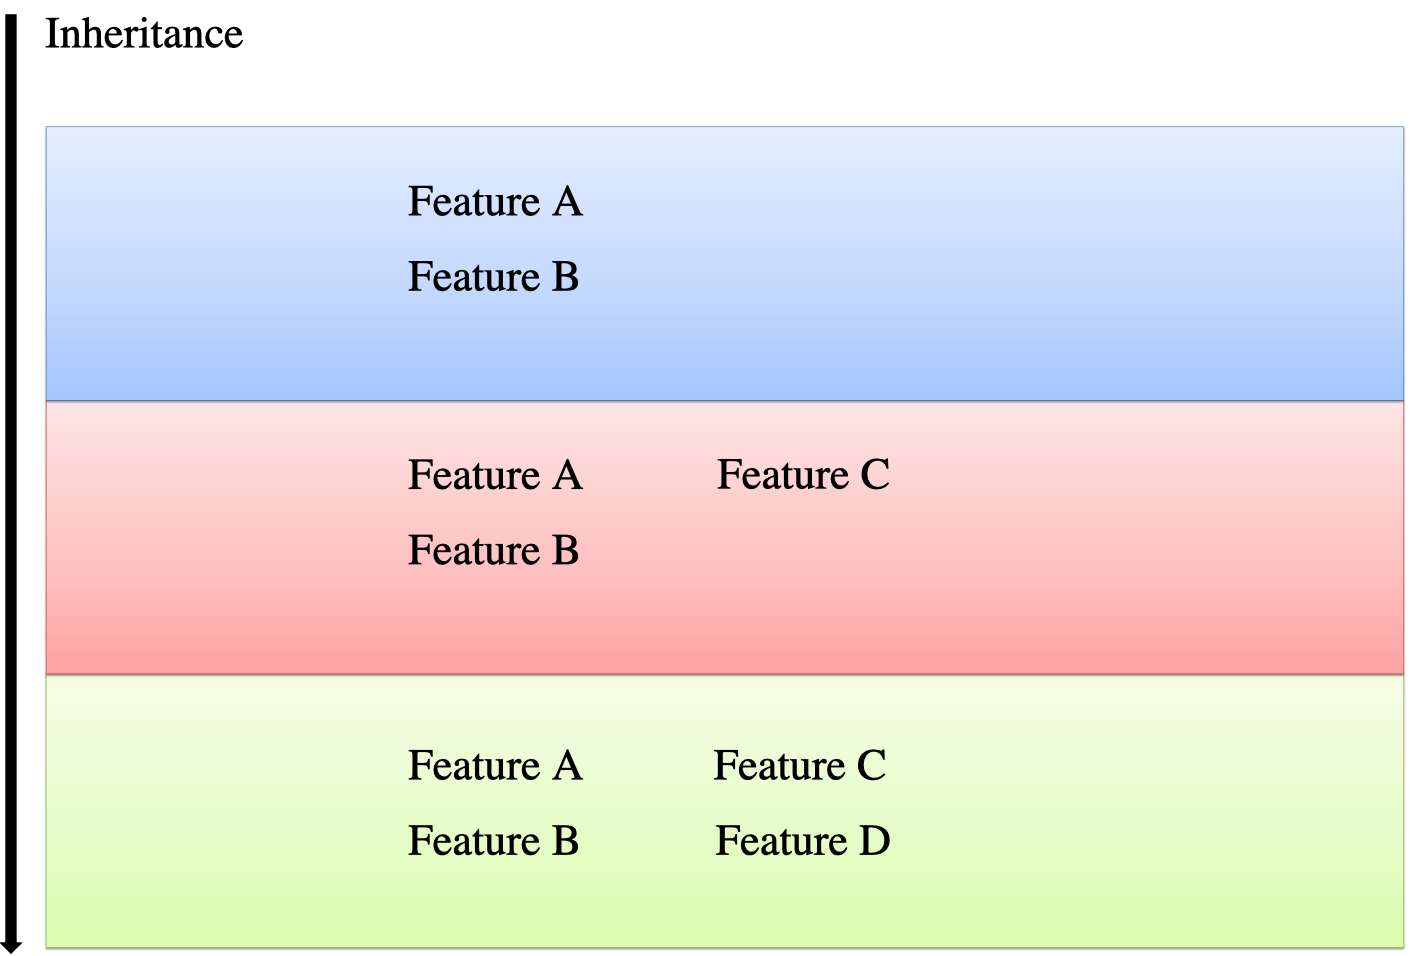
\includegraphics[width=220px]{./images/OopInheritance.png}
\caption{OOP inheritance}
\end{figure}

\begin{itemize}
\item Let’s define one of the fundamental concepts of object programming,
named “inheritance”. Any object bound to a specific level of a class
hierarchy inherits all the traits (as well as the requirements and
qualities) defined inside any of the superclasses. The object’s home
class may define new traits (as well as requirements and qualities)
which will be inherited by any of its superclasses.

\item Inheritance is a common practice (in object programming) of passing
attributes and methods from the superclass (defined and existing) to
a newly created class, called the subclass.

\item The most important factor of the process is the relation between the
superclass and all of its subclasses (note: if B is a subclass of A
and C is a subclass of B, this also means than C is a subclass of A,
as the relationship is fully transitive).
\end{itemize}

\subsection{Objects Roles}
\label{sec:org409e2f8}
\begin{enumerate}
\item an object has a \textbf{name} that uniquely identifies it within its home
namespace (although there may be some anonymous objects, too)
\item an object has a set of individual \textbf{properties} which make it
original, unique or outstanding (although it’s possible that some
objects may have no properties at all)
\item an object has a set of abilities to perform specific \textbf{activities},
able to change the object itself, or some of the other objects.
\end{enumerate}

\subsection{Classes}
\label{sec:orgf3a1791}
\begin{itemize}
\item The class you define has nothing to do with the object: the
existence of a class does not mean that any of the compatible
objects will automatically be created. The class itself isn’t able
to create an object – you have to create it yourself, and Python
allows you to do this.
\item The definition begins with the keyword class. The keyword is
followed by an identifier which will name the class (note: don’t
confuse it with the object’s name – these are two different
things). Next, you add a colon, as classes, like functions, form
their own nested block. The content inside the block define all the
class’s properties and activities.
\item The \texttt{pass} keyword fills the class with nothing. It doesn’t contain
any methods or properties.
\end{itemize}

\begin{minted}[linenos,firstnumber=1]{python}
class OurClass:
    pass
\end{minted}

\subsection{Object Instantiation}
\label{sec:org4c36293}
\begin{itemize}
\item The newly defined class becomes a tool that is able to create new
objects.
\item The tool has to be used explicitly, on demand.
\item Imagine that you want to create one (exactly one) object of the
\texttt{OurClass} class: 
To do this, you need to assign a variable to store
the newly created object of that class, and create an object at the
same time. Note that the class name tries to pretend that it’s a
function
\item The act of creating an object of the selected class is also called
an \textbf{instantiation} (as the object becomes an instance of the class).
\end{itemize}

\begin{minted}[linenos,firstnumber=1]{python}
ourObject = ourClass()
\end{minted}

\subsubsection{Constructor}
\label{sec:org12e69aa}
A constructor is a special kind of method that Python calls when it
instantiates an object using the definitions found in your
class. Python relies on the constructor to perform tasks such as
initializing (assigning values to) any instance variables that the
object will need when it starts. Constructors can also verify that
there are enough resources for the object and perform any other
start-up task you can think of.

\begin{itemize}
\item The name of a constructor is always the same, \texttt{\_\_init\_\_()}. The
constructor can accept arguments when necessary to create the
object. When you create a class without a constructor, Python
automatically creates a default constructor for you that doesn’t do
anything. Every class must have a constructor, even if it simply
relies on the default constructor.
\item It has to have at least \textbf{one parameter} (we’ll discuss this later);
the parameter is used to represent the newly created object – you
can use the parameter to manipulate the object, and to enrich it
with the needed properties;
\item the obligatory parameter is usually named \texttt{self} – it’s only a
convention, but you should follow it – it simplifies the process of
reading and understanding your code.
\item we’ve used the dotted notation, just like when invoking methods;
this is the general convention for accessing an object’s properties
– you need to name the object, put a dot after it, and specify the
desired property’s name; don’t use parentheses! You don’t want to
invoke a method – you want to access a property;
\item if you set a property’s value for the very first time (like in the
constructor), you are creating it; from that moment on, the object
has got the property and is ready to use its value;
\end{itemize}

\begin{minted}[linenos,firstnumber=1]{python}
class MyClass:
    def __init__(self, Name="there"):
	self.Greeting = Name + "!"

    def SayHello(self):
	    print("Hello {0}".format(self.Greeting))


myInstance = MyClass()
myInstance.SayHello()

shaeInstance = MyClass("SHAE")
shaeInstance.SayHello()
\end{minted}

\begin{verbatim}
Hello there!
Hello SHAE!
\end{verbatim}

\subsubsection{Encapsulation}
\label{sec:orgcadae7a}
When any class component has a name \textbf{starting with two underscores},
it becomes \textbf{private} – this means that it can be accessed only from
within the class. You cannot see it from the outside world. This is
how Python implements the encapsulation concept.

\subsubsection{Methods}
\label{sec:org4d7ec9c}
\begin{itemize}
\item All methods have to have a \texttt{self} parameter as their first
parameter(The self name is only a convention but it's existence is
necessary). It plays the same role as the first constructor parameter.
\item It allows the method to access entities (properties and
activities/methods) carried out by the actual object. \textbf{You cannot
omit it}. Every time Python invokes a method, \textbf{it implicitly sends the
current object as the first argument.}
\item If you want to make a method \textbf{private} you have to name it \textbf{starting
with two underscores} otherwise the method will be \textbf{public}.
\item There is one more requirement – the name must have no more than one
trailing underscore. As no trailing underscores at all fully meets
the requirement, you can assume that the name is acceptable.
\end{itemize}

\newpage
\subsection{Stack}
\label{sec:org73a68bb}

\begin{figure}[htbp]
\centering
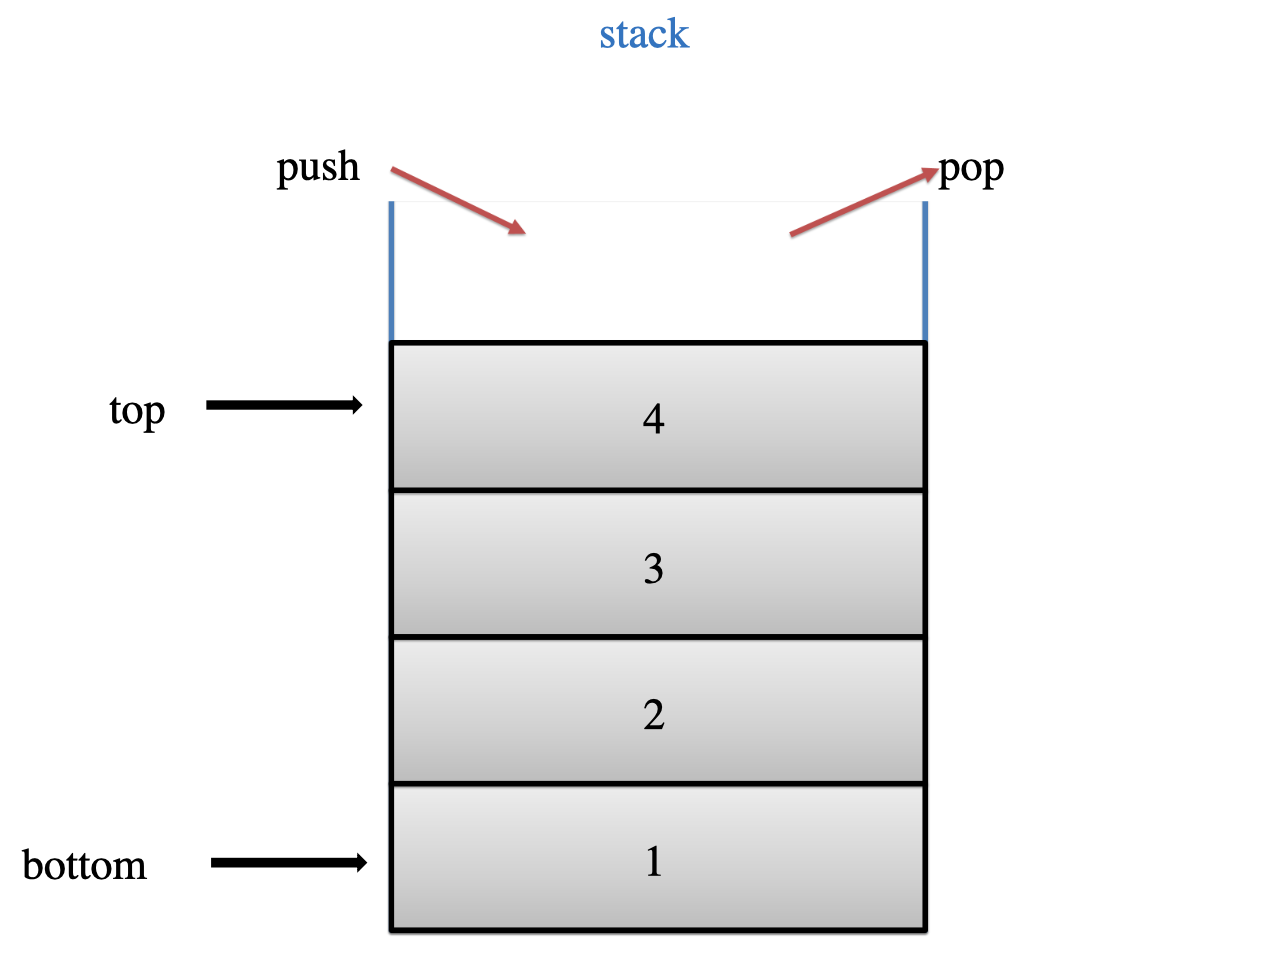
\includegraphics[width=220px]{./images/stack.png}
\caption{Stack}
\end{figure}

\begin{itemize}
\item A stack is a structure developed to store data in a very specific
way. Imagine a stack of coins. You aren’t able to put a coin
anywhere else but on the top of the stack. Similarly, you can’t get
a coin off the stack from any place other than the top of the
stack. If you want to get the coin that lies on the bottom, you have
to remove all the coins from the higher levels.
\item The alternative name for a stack (but only in IT terminology) is
\textbf{LIFO}. It’s an abbreviation for a very clear description of the
stack’s behavior: “Last In – First Out”. The coin that came last
onto the stack will leave first.
\item A stack is an object with two elementary operations, conventionally
named \textbf{\texttt{push}} (when a new element is put on the top) and \textbf{\texttt{pop}} (when an
existing element is taken away from the top).
\item Stacks are used very often in many classical algorithms, and it’s
hard to imagine the implementation of many widely used tools without
the use of stacks.
\end{itemize}

\subsubsection{Procedural Stack}
\label{sec:org17e9c83}
\paragraph{push - pop}
\label{sec:orgc0b2a04}
Here we will define a stack and then \texttt{push} and \texttt{pop} functions. Note
that \texttt{puah} function doesn’t return anything and \texttt{pop} function
doesn’t check if there is any element in the stack.

\begin{minted}[linenos,firstnumber=1]{python}
stack = []

def push(val):
    stack.append(val)

def pop():
    val = stack[-1]
    del stack[-1]
    return val

push(2)
push(2)
push(1)
print(pop())
print(pop())
print(pop())
\end{minted}

\subsubsection{Objective Stack}
\label{sec:org9453f20}
The objective approach delivers very essential pros to stacks like:

\begin{itemize}
\item the ability to \textbf{hide} (protect) selected values against unauthorized
access is called \textbf{encapsulation}; the encapsulated values can be
neither accessed nor modified if you want to use them exclusively;
\item when you have a class implementing all the needed stack behaviors,
you can \textbf{produce as many stacks as you want}; you needn’t copy or
replicate any part of the code;
\item the ability to enrich the stack with new functions comes from
\textbf{inheritance}; you can create a new class (a subclass) which
inherits all the existing traits from the superclass, and adds some
new ones.
\end{itemize}

\paragraph{push - pop}
\label{sec:orge58228a}
Having such a class opens up some new possibilities. For example, you
can now have more than one stack behaving in the same way. Each stack
will have its own copy of private data, but will utilize the same set
of methods.

\begin{minted}[linenos,firstnumber=1]{python}
# This is the class itself 
class Stack:
	def __init__(self):
		self.__stk = []

	def push(self, val):
		self.__stk.append(val)

	def pop(self):
		val = self.__stk[-1]
		del self.__stk[-1]
		return val

\end{minted}


\begin{minted}[linenos,firstnumber=1]{python}
# This is noweb syntax to impart class on org-mode
<<objectiveStack>>

stack = Stack()
stack.push(3)
stack.push(2)
stack.push(1)
print(stack.pop())
print(stack.pop())
print(stack.pop())
print("------------------")
stack1 = Stack()
stack2 = Stack()
stack1.push(3)
stack2.push(stack1.pop())
print(stack2.pop())
\end{minted}

\begin{verbatim}
1
2
3
------------------
3
\end{verbatim}

\newpage
\subsection{Subclasses}
\label{sec:orgf7fc5c7}
\begin{itemize}
\item We don’t want to modify the previously defined stack. It’s already
good enough in its applications, and we don’t want it changed in any
way. \textbf{We want a new stack with new capabilities.} In other words, we
want to construct a subclass of the already existing Stack class.
\item The first step is easy: just define a new subclass pointing to the
class which will be used as the superclass.
\end{itemize}

\texttt{class addingStack(Stack)}

\begin{itemize}
\item The class doesn’t define any new component yet, but that doesn’t
mean that it’s empty. \textbf{It gets all the components defined by its
superclass}

\item Contrary to many other language, \textbf{Python forces you to explicitly
invoke a superclass’ constructor}. Omitting this point will have
harmful effects.
\end{itemize}

\begin{minted}[linenos,firstnumber=1]{python}
class addingStack(Stack):
    def __init__(self):
	Stack.__init__(self)
	self.__sum = 0 
\end{minted}

\begin{itemize}
\item Note the syntax above:
\begin{itemize}
\item you specify the \textbf{superclass’s name} (this is the class whose
constructor you want to run)
\item you put a dot after it;
\item you specify the name of the constructor;
\item you have to point to the object (the class’s instance) which has
to be initialized by the constructor – this is why you have to
specify the argument and use the self variable here; note:
invoking any method (including constructors) from outside the
class never requires you to put the self argument at the
argument’s list – \textbf{invoking a method from within the class demands
explicit usage of the \texttt{self} argument,} and it has to be put first
on the list.
\end{itemize}
\end{itemize}

\subsubsection{Changing functionality of methods}
\label{sec:org42e906b}

\begin{minted}[linenos,firstnumber=1]{python}
def push(self, val):
    self.__sum += val
    Stack.push(self, val)
\end{minted}

Is it really adding? We have these methods in the superclass
already. Can we do something like that? Yes, we can. It means that
we’re going to \textbf{change the functionality of the methods, not their
names.} We can say more precisely that the interface (the way in which
the objects are handled) of the class remains the same when changing
the implementation at the same time.

\emph{Note:} the second activity has already been implemented inside the
superclass – so we can use that. Furthermore, we have to use it, as
there’s no other way to access the \texttt{\_\_stk} variable.

Note the way we’ve invoked the previous implementation of the push
method (the one available in the superclass):
\begin{itemize}
\item we have to specify the superclass’s name; this is necessary in order
to clearly indicate the class containing the method, to avoid
confusing it with any other function of the same name;
\item we have to specify the target object and to pass it as the first
argument (it’s not implicitly added to the invocation in this
context)
\end{itemize}

We say that the \texttt{push} method has been overridden – the same name as
in the superclass now represents a different functionality.

\begin{minted}[linenos,firstnumber=1]{python}
# This is noweb syntax to impart class on org-mode
<<objectiveStack>>

class AddingStack(Stack):
        def __init__(self):
                Stack.__init__(self)
                self.__sum = 0

        def getSum(self):
                return self.__sum

        def push(self, val):
                self.__sum += val
                Stack.push(self,val)

        def pop(self):
                val = Stack.pop(self)
                self.__sum -= val
                return val

stack = AddingStack()
for i in range(5):
        stack.push(i)
print(stack.getSum())
print("------------------")
for i in range(5):
        print(stack.pop())
\end{minted}

\begin{verbatim}
10
------------------
4
3
2
1
0
\end{verbatim}

\subsection{Instance variable}
\label{sec:orgd02989e}
Object-oriented programming allows for variables to be used at the
\textbf{class level} or the \textbf{instance level}. Variables are essentially
symbols that stand in for a value you’re using in a program. At the
class level, variables are referred to as class variables, whereas
variables at the instance level are called instance variables.

When we expect variables are going to be consistent across instances,
or when we would like to initialize a variable, we can define that
variable at the class level. When we anticipate the variables will
change significantly across instances, we can define them at the
instance level.

Python objects, when created, are gifted with a small set of
predefined properties and methods. Each object has got them, whether
you want them or not. One of them is a variable named \texttt{\_\_dict\_\_} (it’s a
dictionary).  The variable contains the names and values of all the
properties (variables) the object is currently carrying. Let’s make
use of it to safely present an object’s contents.

\begin{minted}[linenos,firstnumber=1]{python}
class Class:
	def __init__(self, val=1):
		self.First = val

	def setSecond(self, val=2):
		self.Second = val


object1 = Class()
object2 = Class(2)
object2.setSecond(3)
object3 = Class(4)
object3.Third = 5


print(object1.__dict__)
print(object2.__dict__)
print(object3.__dict__)
\end{minted}

\begin{verbatim}
{'First': 1}
{'First': 2, 'Second': 3}
{'First': 4, 'Third': 5}
\end{verbatim}

\begin{itemize}
\item the class named Class has a constructor, which unconditionally
creates an instance variable named First, and sets it with the value
passed through the first argument (from the class user’s
perspective) or the second argument (from the constructor’s
perspective); note the default value of the parameter – any trick
you can do with a regular function parameter can be applied to
methods, too;
\item the class also has a method which creates another instance variable,
named Second;
\item we’ve created three objects of the class Class, but all these
instances differ:
\begin{itemize}
\item object1 only has the property named First;
\item object2 has two properties: First and Second;
\item object3 has been enriched with a property named Third just on the
fly, outside the class’s code – this is possible and fully
permissible.
\end{itemize}
\end{itemize}

\emph{\textbf{Important}}: modifying an instance variable of any object has \textbf{no
impact} to all the remaining objects. Instance variables are perfectly
isolated from each other.

\subsubsection{mangling}
\label{sec:orgcf475a8}
In Python, mangling is used for "private" class members which are
designated as such by giving them a name with two leading underscores
and no more than one trailing underscore.

\begin{minted}[linenos,firstnumber=1]{python}
class Class:
	def __init__(self, val=1):
		self.__First = val

	def setSecond(self, val=2):
		self.__Second = val


object1 = Class()
object2 = Class(2)
object2.setSecond(3)
object3 = Class(4)
object3.__Third = 5


print(object1.__dict__)
print(object2.__dict__)
print(object3.__dict__)
print(object1._Class__First)
\end{minted}

\begin{verbatim}
{'_Class__First': 1}
{'_Class__First': 2, '_Class__Second': 3}
{'_Class__First': 4, '__Third': 5}
1
\end{verbatim}

It’s nearly the same as the previous one. The only difference is in
the property names. We’ve added two underscores in front of them. As
you know, such an addition makes the instance variable private – it
becomes inaccessible from the outer world.

When Python sees that you want to add an instance variable to an
object and you’re going to do it inside any of the object’s methods,
it \textbf{mangles} the operation in the following way:
\begin{itemize}
\item it puts a class name before your name;
\item it puts an additional underscore at the beginning.
\end{itemize}

This is why the \textbf{\texttt{\_\_First}} becomes \textbf{\texttt{\_Class\_\_First}}. The name is now fully
accessible from outside the class. You can run a code like this:
\begin{itemize}
\item \texttt{print(object1.\_Class\_\_First)}

\newpage
\end{itemize}

\subsection{Class variable}
\label{sec:org6a1312e}
A class variable is a property which exists in just one copy and is
stored outside any object. \textbf{initializing the variable inside the class
but outside any of its methods makes the variable a class variable;}

\begin{minted}[linenos,firstnumber=1]{python}
class Class:

	Counter = 0

	def __init__(self, val=1):
		self.__First = val
		Class.Counter += 1


object1 = Class()
print(object1.__dict__, object1.Counter)
print("--------------------")

object2 = Class(2)
object3 = Class(4)
print(object1.__dict__, object1.Counter)
print(object2.__dict__, object2.Counter)
print(object3.__dict__, object3.Counter)

\end{minted}

\begin{verbatim}
{'_Class__First': 1} 1
--------------------
{'_Class__First': 1} 3
{'_Class__First': 2} 3
{'_Class__First': 4} 3
\end{verbatim}

\textbf{Notes}:
\begin{itemize}
\item class variables aren’t shown in an object’s \texttt{\_\_dict\_\_} (this is
natural as class variables aren’t parts of an object) but you can
always try to look into the variable of the same name, but at the
class level – we’ll show you this very soon;
\item a class variable always presents the same value in all class
instances (objects)
\end{itemize}

Mangling a class variable’s name has the same effects as those you’re
already familiar with.

\begin{minted}[linenos,firstnumber=1]{python}
class Class:
	__Counter = 0

	def __init__(self, val=1):
		self.__First = val
		Class.__Counter += 1


object1 = Class()
object2 = Class(2)
object3 = Class(4)

print(object1.__dict__, object1._Class__Counter)
print(object2.__dict__, object2._Class__Counter)
print(object3.__dict__, object3._Class__Counter)

\end{minted}

\begin{verbatim}
{'_Class__First': 1} 3
{'_Class__First': 2} 3
{'_Class__First': 4} 3
\end{verbatim}


\newpage

\subsection{\texttt{hasattr}}
\label{sec:org1ab997c}
Python provides a function which is able to safely check if any
object/class contains a specified property. The function is named
hasattr, and expects two arguments to be passed to it:
\begin{itemize}
\item the \textbf{class or the object} being checked;
\item the \textbf{name of the property} whose existence has to be reported (\emph{note:}
\emph{it has to be a string containing the attribute name, not the name}
\emph{alone})
\item Don’t forget that the hasattr() function can operate on classes,
too. You can use it to find out if a class variable is available
\end{itemize}

\begin{minted}[linenos,firstnumber=1]{python}
class Class:
	Attr = 1

	def __init__(self, val):
		if val % 2 != 0:
			self.a = 1
		else:
			self.b = 2


object = Class(1)
if hasattr(object, 'a'):
	print(object.a)
else:
	print(object.b)

print("-------------------")

print(hasattr(Class, 'Attr'))
print(hasattr(Class, 'pop'))

\end{minted}

\begin{verbatim}
1
-------------------
True
False
\end{verbatim}

\break
\newline

Another useful example:

\begin{minted}[linenos,firstnumber=1]{python}
class Class:
	a = 1

	def __init__(self):
		self.b = 2


object = Class()
print(hasattr(object,'b'))
print(hasattr(object,'a'))
print(hasattr(Class,'b'))
print(hasattr(Class,'a'))

\end{minted}

\begin{verbatim}
True
True
False
True
\end{verbatim}
\newpage

\subsection{Classes methods}
\label{sec:org3a7deb9}
A method is a function embedded inside a class. There is one
fundamental requirement – a method is obliged to have at least one
parameter (there are no such thing as parameterless method – a method
may be invoked without an argument, but not declared without
parameters). The first (or only) parameter is usually named
\texttt{self}. The name \texttt{self} suggests the parameter’s purpose – it
identifies the object for which the method is invoked. 

\begin{itemize}
\item The \texttt{self} parameter is used to obtain access to the object’s
instance and class variables.
\end{itemize}

\begin{minted}[linenos,firstnumber=1]{python}
class Class:
    Variable = 3

    def method(self):
	print(self.Variable, self.var)


obj = Class()
obj.var = 4
obj.method()
\end{minted}

\begin{verbatim}
3 4
\end{verbatim}

\vspace{10 mm}

\begin{itemize}
\item The \texttt{self} parameter is also used to invoke other object/class methods
from inside the class.
\end{itemize}

\begin{minted}[linenos,firstnumber=1]{python}
class Class:
    def other(self):
	print("Other")

    def method(self):
	print("Method")
	self.other() 


obj = Class()
obj.method()
\end{minted}

\begin{verbatim}
Method
Other
\end{verbatim}

\vspace{10 mm}

\begin{itemize}
\item If you name a method \texttt{\_\_init\_\_}, it won’t be a regular method – \textbf{it
will be a constructor.} If a class has a constructor, *it is invoked
automatically and implicitly when the object of the class is
instantiated.*

Note that the constructor:

\begin{itemize}
\item cannot return a value,as it is designed to return a newly created
object and nothing else;

\item cannot be invoked directly either from the object or from inside the
class (you can invoke a constructor from any of the object’s
superclasses, but we’ll discuss this issue later).
\end{itemize}

\begin{minted}[linenos,firstnumber=1]{python}
class Class:

    def __init__(self, val):
	self.var = val


obj = Class(5)
print(obj.var)
\end{minted}

\begin{verbatim}
5
\end{verbatim}
\end{itemize}

\vspace{10 mm}

\begin{itemize}
\item Everything we’ve said about property name mangling applies to method
names, too – a method whose name starts with \_\_ is (partially)
hidden.
\end{itemize}

\begin{minted}[linenos,firstnumber=1]{python}
class Class:

    def visible(self):
	print("Visible")

    def __hidden(self):
	print("Hidden")


obj = Class()
obj.visible()

try:
    obj.__hidden()
except:
    print("Failed")

obj._Class__hidden()

\end{minted}

\begin{verbatim}
Visible
Failed
Hidden
\end{verbatim}
\subsection{Introspection/Reflection}
\label{sec:org3ad7f76}
\begin{itemize}
\item \textbf{Introspection}, which is the ability of a program to examine the
type or properties of an object at runtime;
\item \textbf{Reflection}, which goes a step further, and is the ability of a
program to manipulate the values, properties and/or functions of an
object at runtime.
\end{itemize}

In other words, you don’t have to know a complete class/object
definition to manipulate the object, as the object and/or its class
contain the metadata allowing you to recognize its features during
program execution.

\subsubsection{\texttt{\_\_name\_\_}}
\label{sec:orgc537964}
The property contains the name of the class. It’s a string. the
\texttt{\_\_name\_\_} attribute is absent from the object – \textbf{it exists only inside
classes.}

If you want to find the class of a particular object, you can use a
function named \texttt{type()}, which is able (among other things) to find a
class which has been used to instantiate any object.

\begin{minted}[linenos,firstnumber=1]{python}
class Classy:
	pass


print(Classy.__name__)
obj = Classy()
print(type(obj).__name__)
\end{minted}

\begin{verbatim}
Classy
Classy
\end{verbatim}

\subsubsection{\texttt{\_\_module\_\_}}
\label{sec:org7335742}
\texttt{\_\_module\_\_} is a string, too – it stores the name of the module which
contains the definition of the class.

\begin{minted}[linenos,firstnumber=1]{python}
class Classy:
    pass


print(Classy.__module__)
obj = Classy()
print(obj.__module__)
\end{minted}

\begin{verbatim}
__main__
__main__
\end{verbatim}

As you know, any module named \texttt{\_\_main\_\_} is actually not a module, but
the file currently being run.

\subsubsection{\texttt{\_\_base\_\_}}
\label{sec:org0f7c601}
\texttt{\_\_bases\_\_} is a tuple. The tuple contains classes (not class names)
which are direct superclasses for the class. The order is the same as
that used inside the class definition.

\begin{minted}[linenos,firstnumber=1]{python}
class Super1:
	pass


class Super2:
	pass


class Sub(Super1, Super2):
	pass


def printbases(cls):
	print('( ', end='')
	for x in cls.__bases__:
		print(x.__name__, end=' ')
	print(')')


printbases(Super1)
printbases(Super2)
printbases(Sub)

\end{minted}

\begin{verbatim}
( object )
( object )
( Super1 Super2 )
\end{verbatim}
\subsection{Internal object identifier}
\label{sec:org5c91e4b}
if you run the code 

\texttt{print(objectName)}

then you will see something like

\texttt{<\_\_main\_\_.Star object at 0x7f1074cc7c50>}

in which the \texttt{0x7f1074cc7c50} is the \textbf{internal object identifier}

\subsection{\texttt{\_\_str\_\_}}
\label{sec:orgf555569}
When Python needs any class/object to be presented as a string
(putting an object as an argument in the \texttt{print()} function invocation
fits this condition) it tries to invoke a method named \texttt{\_\_str\_\_()}
from the object and to use the string it returns. The default
\texttt{\_\_str\_\_()} method returns something like \texttt{<\_\_main\_\_.Star object at
0x7f1074cc7c50>} – ugly and not very informative. You can change it
just by defining your own method of the name.

\begin{minted}[linenos,firstnumber=1]{python}
class Star:
	def __init__(self,  name,  galaxy):
		self.name = name
		self.galaxy = galaxy

	def __str__(self):
		return self.name + ' in ' + self.galaxy


sun = Star("Sun", "Milky Way")
print(sun)

\end{minted}

\begin{verbatim}
Sun in Milky Way
\end{verbatim}
\newpage

\subsection{\texttt{issubclass}}
\label{sec:orgd0cb2e7}
Python offers a function which is able to identify a relationship
between two classes, and although its diagnosis isn’t complex, it can
check if a particular class is a subclass of any other class.

\texttt{issubclass(class1, class2)}

The function returns True if class1 is a subclass of class2, and False
otherwise.

There is one important observation to make: each class is considered
to be a subclass of itself.

\begin{minted}[linenos,firstnumber=1]{python}
class Vehicle:
	pass


class LandVehicle(Vehicle):
	pass


class TrackedVehicle(LandVehicle):
	pass


for cl1 in [Vehicle, LandVehicle, TrackedVehicle]:
	for cl2 in [Vehicle, LandVehicle, TrackedVehicle]:
		print(issubclass(cl1,cl2),end='\t')
	print()

\end{minted}

\textbf{Code Result:}

\begin{figure}[htbp]
\centering
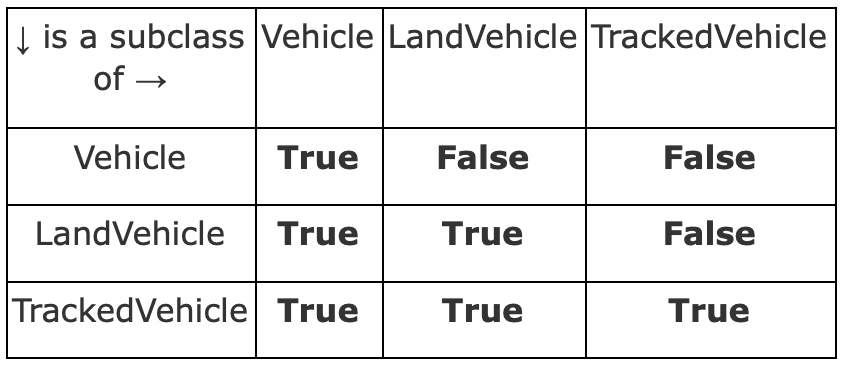
\includegraphics[width=230px]{./images/subclasses.png}
\caption{Result table}
\end{figure}
\subsection{instance vs variables}
\label{sec:org0bfa1a9}
Variables don’t store the objects themselves, but only the handles
pointing to the internal Python memory. Assigning a value of an object
variable to another variable doesn’t copy the object, but only its
handle. This is why an operator like \texttt{is} may be very useful in
particular circumstances. he operator checks whether two variables
(object1 and object2 here) refer to the same object.

\texttt{object1 is object2}
\vspace{10 mm}

\textbf{Sample code:}

\begin{minted}[linenos,firstnumber=1]{python}
class ThisIsClass:
	def __init__(self, val):
		self.val = val


ob1 = ThisIsClass(0)
ob2 = ThisIsClass(2)
ob3 = ob1
ob3.val += 1
print(ob1 is ob2)
print(ob2 is ob3)
print(ob3 is ob1)
print(ob1.val, ob2.val, ob3.val)

str1 = "Mary had a little "
str2 = "Mary had a little lamb"
str1 += "lamb"
print(str1 == str2, str1 is str2)

\end{minted}

\begin{verbatim}
False
False
True
1 2 1
True False
\end{verbatim}

\begin{itemize}
\item \textbf{Code Description}: There is a very simple class equipped with a
simple constructor, creating just one property. The class is used to
instantiate two objects. The former is then assigned to another
variable, and its val property is incremented by one.  Afterward,
the is operator is applied three times to check all possible pairs
of objects, and all val property values are also printed. The last
part of the code carries out another experiment. After three
assignments, both strings contain the same texts, but these texts
are stored in different objects.
\end{itemize}
\subsection{Override}
\label{sec:orga637e4f}

See the code below:

\begin{minted}[linenos,firstnumber=1]{python}
class Level0:
	Var = 100

	def fun(self):
		return 101

class Level1(Level0):
	Var = 200

	def fun(self):
		return 201

class Level2(Level1):
	pass


object = Level2()
print(object.Var, object.fun())

\end{minted}

\begin{verbatim}
200 201
\end{verbatim}

\textbf{Code Description:} Both, Level0 and Level1 classes define a method
 named \textbf{fun()} and a property named \textbf{Var}. As you can see, the Var
 class variable and \textbf{fun()} method from Level1 class \textbf{override the
 entities of the same names} derived from the Level0 class.

\subsection{How python treat classes}
\label{sec:org6085519}
\begin{itemize}
\item When you try to access any object’s entity, Python will try (in this
order):

\begin{enumerate}
\item to find it inside the object itself;
\item to find it in all classes involved in the object’s inheritance
line from bottom to top;
\item if both of the above fail, an exception (\textbf{AttributeError}) is
raised.
\end{enumerate}
\end{itemize}


\begin{itemize}
\item If a subClass has more than one superClass, python treats it in this
order:

\begin{enumerate}
\item inside the object itself;
\item in its superclasses, from bottom to top;
\item if there is more than one class on a particular inheritance path,
Python scans them from left to right.

\begin{minted}[linenos,firstnumber=1]{python}
class Level0:
	Var = 100

	def fun(self):
		return 101


class Level1(Level0):
	Var = 200

	def fun(self):
		return 201


class Level2(Level1):
	pass


object = Level2()
print(object.Var, object.fun())

\end{minted}

\begin{verbatim}
200 201
\end{verbatim}
\end{enumerate}
\end{itemize}
\subsection{polymorphism}
\label{sec:org42a1f4d}

the situation in which the subclass is able to modify its superclass
behavior (just like in the example below) is called polymorphism. The
word comes from Greek (polys: “many, much” and morphē, “form, shape”),
which means that \textbf{one and the same class can take various forms}
depending on the redefinitions done by any of its subclasses. The
method, redefined in any of the superclasses, thus changing the
behavior of the superclass, is called \textbf{virtual}. In other words, \textbf{no}
\textbf{class is given once and for all}. Each class’s behavior may be modified
at any time by any of its subclasses.


 \textbf{Example:} There are two classes, named \textbf{One} and \textbf{Two}, while \textbf{Two}
is derived from \textbf{One}. Nothing special. However, one thing looks
remarkable – the \textbf{doit()} method. It’s defined twice: originally
inside \textbf{One} and subsequently inside \textbf{Two}. The essence of the example
lies in the fact that it is invoked just once – inside \textbf{One}.
\textbf{The second invocation will launch \texttt{doit()} in the form existing inside the \texttt{Two}.}

\begin{minted}[linenos,firstnumber=1]{python}
class One:
	def doit(self):
		print("doit from One")
	def doanything(self):
		self.doit()


class Two(One):
	def doit(self):
		print("doit from Two")


one = One()
two = Two()

one.doanything()
two.doanything()
\end{minted}

\begin{verbatim}
doit from One
doit from Two
\end{verbatim}
\subsection{Composition}
\label{sec:orgfbeab50}
Composition is the process of \textbf{composing an object using other}
\textbf{different objects}. The objects used in the composition deliver a set
of desired traits (properties and/or methods) so we can say that they
act like blocks used to build a more complicated structure.
It can be said that:

\begin{itemize}
\item \textbf{Inheritance} extends a class’s capabilities by adding new
components and modifying existing ones; in other words, the complete
recipe is contained inside the class itself and all its ancestors;
the object takes all the class’s belongings and makes use of them;
\item \textbf{Composition} projects a class as a container able to store and use
other objects (derived from other classes) where each of the objects
implements a \textbf{part of a desired class’s behavior.}
\end{itemize}

\begin{minted}[linenos,firstnumber=1]{python}
import time


class Tracks:
	def changedirection(self, left, on):
		print("tracks: ", left, on)


class Wheels:
	def changedirection(self, left, on):
		print("wheels: ", left, on)


class Vehicle:
	def __init__(self, controller):
		self.controller = controller

	def turn(self, left):
		self.controller.changedirection(left, True)
		time.sleep(0.25)
		self.controller.changedirection(left, False)


wheeled = Vehicle(Wheels())
tracked = Vehicle(Tracks())

wheeled.turn(True)
tracked.turn(False)

\end{minted}

\begin{verbatim}
wheels:  True True
wheels:  True False
tracks:  False True
tracks:  False False
\end{verbatim}

\newpage

\section{Working with files}
\label{sec:org5dd8699}
\subsection{Addressing}
\label{sec:org51555da}
Python is smart enough to be able to convert slashes into backslashes
each time it discovers that it’s required by the OS. This means that
any the following assignments will work with Windows, too:

\texttt{name = "/dir/file"}

\texttt{name = "c:/dir/file"}

\subsection{Open Modes}
\label{sec:orgb036264}
To connect (bind) the stream with the file, it’s necessary to perform
an explicit operation.  The operation of connecting the stream with a
file is called opening the file, while disconnecting this link is
named closing the file.  Hence, the conclusion is that the very first
operation performed on the stream is always open and the last one is
close. The program, in effect, is free to manipulate the stream
between these two events and to handle the associated file. The
opening of the stream is not only associated with the file, but should
also declare the manner in which the stream will be processed. This
declaration is called an \textbf{open mode.} There are three basic modes used
to open the stream:

\begin{itemize}
\item \textbf{read mode:} a stream opened in this mode allows read operations
only; trying to write to the stream will cause an exception (the
exception is named \texttt{UnsupportedOperation}, which inherits \texttt{OSError}
and \texttt{ValueError}, and comes from the \texttt{io} module); the file
associated with the stream must exist and has to be readable,
otherwise open() function raises exception.

\item \textbf{write mode:} a stream opened in this mode allows write operations
only; attempting to read the stream will cause the exception
mentioned above; the file associated with the stream doesn't need to
exist; if it doesn't exist it will be created; if it exists it will
truncated to the length of zero (erased); if the creation isn't
possible (e.g. due to system permissions) the open() function raises
an exception

\item \textbf{update mode}: a stream opened in this mode allows both writes and
reads. the file associated with the stream doesn't need to exist; if
it doesn't exist it will be created; if it exists the virtual
recording head will be set at the end of the file (the previous
content of the file remains untouched)
\end{itemize}

\textbf{Notes:}
\begin{itemize}
\item If you open the stream with \texttt{r+}:
\begin{itemize}
\item the stream will be opened in “read and update” mode;
\item The file associated with the stream must exist and has to be
writeable, otherwise the open() function raises an exception
\item both read and write operations are allowed for the stream
\end{itemize}
\end{itemize}


\begin{itemize}
\item If you open the stream with \texttt{w+}:
\begin{itemize}
\item the stream will be opened in “write and update” mode;
\item the file associated with the stream doesn't need to exist; if it
doesn't exist it will be created; the previous content of the file
remains untouched
\item both read and write operations are allowed for the stream
\end{itemize}
\end{itemize}

\newpage

\subsection{I/O}
\label{sec:orgd39d773}
When you read something from a stream, a virtual head moves over the
stream according to the number of bytes transferred from the stream.
When you write something to the stream, the same head moves along the
stream recording the data from the memory.  Whenever we talk about
reading from and writing to the stream, try to imagine this
analogy. The programming books refer to this mechanism as the \textbf{current}
\textbf{file position}, and we’ll also use this term

An object of an adequate class is created when you open the file and
annihilate it at the time of closing.  Between these two events, you
can use the object to specify what operations should be performed on a
particular stream. The operations you’re allowed to use are imposed by
the way in which you’ve opened the file.  In general, the object comes
from one of the classes shown here: 

\begin{figure}[htbp]
\centering
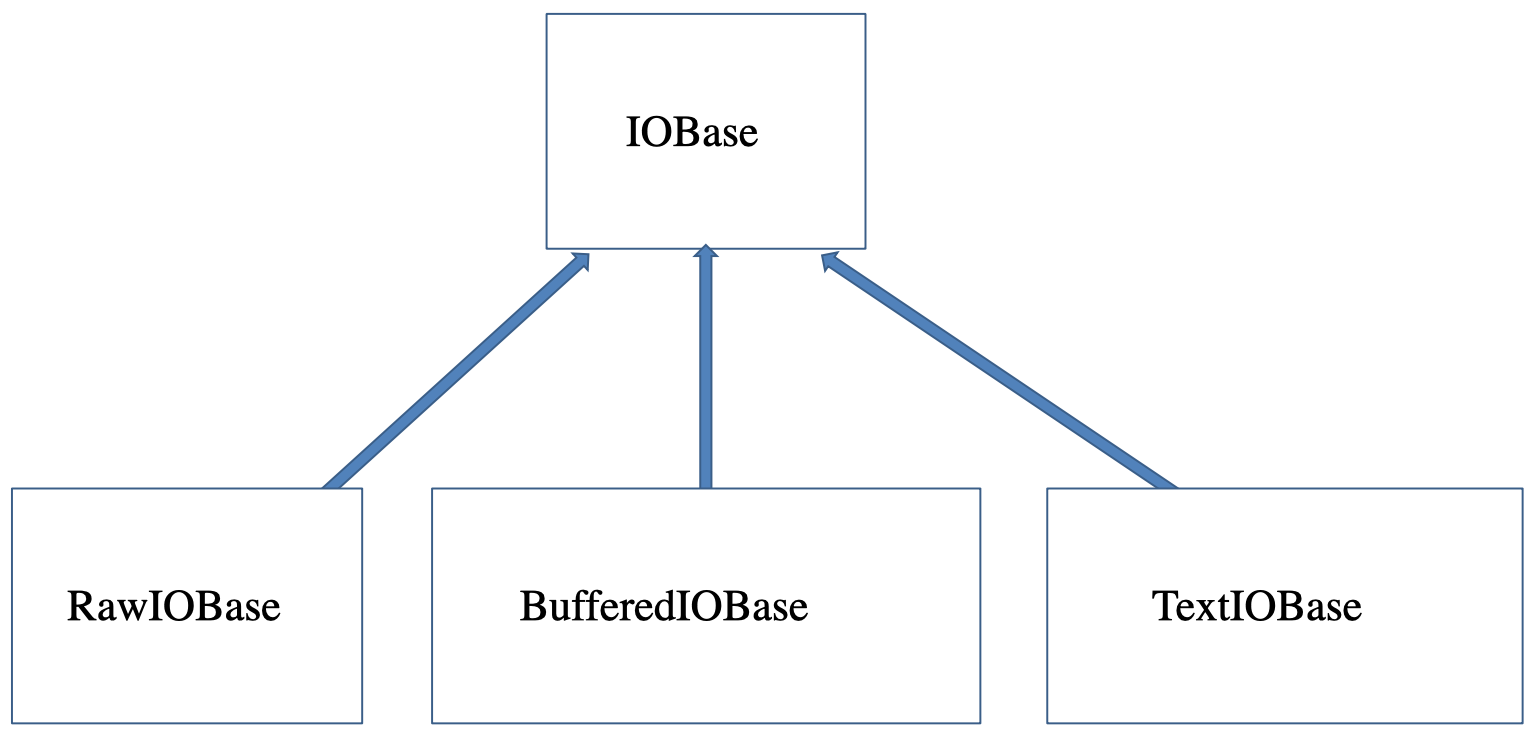
\includegraphics[width=230px]{./images/IO.png}
\caption{I/O Classes}
\end{figure}

If you want to get rid of the object, you invoke the method named
\texttt{close()}. The invocation will sever the connection to the object, and
the file and will remove the object.

\newpage

\subsubsection{Reading files}
\label{sec:org4c13e26}
\begin{itemize}
\item \textbf{Text File}: These ones are structured in lines; that is, they contain
typographical characters (letters, digits, punctuation, etc.)
arranged in rows (lines), as seen with the naked eye when you look
at the contents of the file in the editor.  This file is written (or
read) mostly \textbf{character by character, or line by line.}
\item \textbf{Others}: The former files don’t contain text but a sequence of
bytes of any value. This sequence can be, for example, an executable
program, an image, an audio or a video clip, a database file,
etc. Because these files don’t contain lines, the reads and writes
relate to portions of data of any size. Hence the data is
\textbf{read/written byte by byte, or block by block, where the size of the}
\textbf{block usually ranges from one to an arbitrarily chosen value.}
\end{itemize}

\subsubsection{End-OF-Line issue}
\label{sec:org79d77e9}
Since portability issues were (and still are) very serious, a decision
was made to definitely resolve the issue in a way that doesn’t engage
the developer’s attention.

\begin{itemize}
\item when the stream is open and it’s advised that the data in the
associated file will be processed as text (or there is no such
advisory at all), it is switched into text mode;

\item during reading/writing of lines from/to the associated file, nothing
special occurs in the Unix environment, but when the same operations
are performed in the Windows environment, a process called a
\textbf{translation of newline characters} occurs: when you read a line from
the file, every pair of \texttt{\textbackslash{}r\textbackslash{}n} characters is replaced with a single \texttt{\textbackslash{}n}
character, and vice versa; during write operations, every \texttt{\textbackslash{}n}
character is replaced with a pair of \texttt{\textbackslash{}r\textbackslash{}n} characters;

\item the mechanism is completely transparent to the program, which can be
written as if it was intended for processing Unix/Linux text files
only; the source code run in a Windows environment will work
properly, too;

\item when the stream is open and it’s advised to do so, its contents are
taken as-is, without any conversion – no bytes are added or omitted.
\end{itemize}




\newpage

\subsection{Error handling}
\label{sec:org736c5a4}
Fortunately, there is a function that can dramatically simplify the
error handling code. It’s named \texttt{strerror()}, it comes from \texttt{os} module
and expects just one argument – an error number.  Its role is simple:
you give an error number and get a string describing the meaning of
the error.  Note: if you pass a non-existent error code (a number
which is not bound to any actual error), the function will raise
\texttt{ValueError} exception.

\begin{minted}[linenos,firstnumber=1]{python}
from os import strerror
try: 
	stream = open("path/to/file","rt")
	# actual processing goes here
	stream.close()
except Exception as exc:
	print("File could not be opened:",strerror(exc.errno))
\end{minted}

\subsection{\texttt{read()}}
\label{sec:orgf4b3b6e}
If applied to a text file, the function is able to:

\begin{itemize}
\item read a desired number of characters (including just one) from the
file, and return them as a string;
\item read all the file contents, and return them as a string;
\item if there is nothing more to read (the virtual reading head reaches
the end of the file), the function \textbf{returns} an \textbf{empty string}.
\item \texttt{read()} function, invoked without any arguments or with an argument
that evaluates to \texttt{None}, will read the hole file as once. Pay
attention, doing so for a big file could corrupt your OS.
\end{itemize}


\begin{minted}[linenos,firstnumber=1]{python}
from os import strerror
try:
	cnt = 0
	s = open('text.txt',"rt")
	ch = s.read(1)
	while ch != '':
		cnt += 1
		ch = s.read(1)
	s.close()
	print("Characters in file:", cnt)
except IOError as e:
	print("I/O error occurred: ", strerror(e.errno))
\end{minted}

\begin{verbatim}
Characters in file: 446
\end{verbatim}

\subsection{\texttt{readline()}}
\label{sec:org4290d15}
If you want to treat the file’s contents as a set of lines, not a
bunch of characters, the \textbf{readline()} method will help you with that.
The method tries to read a complete line of text from the file, and
returns it as a string in the case of success. Otherwise, it returns
an \textbf{empty string.}

\begin{minted}[linenos,firstnumber=1]{python}
from os import strerror
try:
	ccnt = lcnt = 0
	s = open('text.txt','rt')
	line = s.readline()
	while line != '':
		lcnt += 1
		for ch in line:
			ccnt += 1
		line = s.readline()
	s.close()
	print("Characters in file:", ccnt)
	print("Lines in file:     ", lcnt)
except IOError as e:
	print("I/O error occurred: ", strerr(e.errno))
\end{minted}

\begin{verbatim}
Characters in file: 446
Lines in file:      7
\end{verbatim}

\subsection{\texttt{readlines()}}
\label{sec:org38c01e0}
The \texttt{readlines()} method, when invoked without arguments, tries to
read all the file contents, and \textbf{returns a list of strings, one}
\textbf{element per file line.} If you’re not sure that the file size is
small enough and don’t want to test the OS, you can convince the
\texttt{readlines()} method to read \textbf{not more than a specified number of
bytes} at once (the returning value remains the same – it’s a list of
a string).  The maximum accepted input buffer size is passed to the
method as its argument. Note that when there is nothing to read from
the file, the method returns an \textbf{empty list}. Use it, for instance
it's length to detect the end of the file.


\begin{minted}[linenos,firstnumber=1]{python}
from os import strerror
try:
	ccnt = lcnt = 0
	s = open('text.txt','rt')
	lines = s.readlines(20)
	while len(lines) != 0:
		for line in lines:
			lcnt += 1
			for ch in line:
				ccnt += 1
		lines = s.readline(10)
	s.close()
	print("Characters in file:", ccnt)
	print("Lines in file:     ", lcnt)
except IOError as e:
	print("I/O error occurred: ", strerr(e.errno))
\end{minted}

\begin{verbatim}
Characters in file: 446
Lines in file:      383
\end{verbatim}

\vspace{10 mm}

\subsection{\texttt{write()}}
\label{sec:orgd38405a}
Writing text files seems to be simpler, as in fact there is one method
that can be used to perform such a task.  The method is named
\texttt{write()} and it expects just one argument – a string that will be
transferred to an open file (don’t forget – the open mode should
reflect the way in which the data is transferred – writing a file
opened in read mode won’t succeed).  No newline character is added to
the \textasciitilde{}write()\textasciitilde{}’s argument, so you have to add it yourself if you want
the file to be filled with a number of lines. We’ve decided to write
the string’s contents character by character (this is done by the
inner for loop) but you’re not obliged to do it in this way. We just
wanted to show you that \texttt{write()} is able to operate on single
characters.

\begin{minted}[linenos,firstnumber=1]{python}
from os import strerror
try:
	fo = open('newtext.txt','wt')
	for i in range(10):
		s = "#" + str(i+1) + " "
		for ch in s:
			fo.write(ch)
	fo.close()
except IOError as e:
	print("I/O error occurred: ", strerr(e.errno))

try:
    stream = open('newtext.txt', "rt")
    print(stream.read())
except Exception as e:
	print("I/O error eccurred: ", strerr(e.errno))


\end{minted}

\begin{verbatim}
#1 #2 #3 #4 #5 #6 #7 #8 #9 #10 
\end{verbatim}

\subsubsection{Write to stderr}
\label{sec:org0ae8584}
You can use the same method to write to the \texttt{stderr} stream, but
don’t try to open it, as it’s always open implicitly. For example, if
you want to send a message string to stderr to distinguish it from
normal program output, it may look like this:

\begin{minted}[linenos,firstnumber=1]{python}
import sys
sys.stderr.write("Error message")
\end{minted}


\newpage

\subsection{Amorphous data}
\label{sec:org6c7088e}
Amorphous data is data which have no specific shape or form – they are
just a series of bytes. The most important aspect of this is that in
the place where we have contact with the data, we are not able to, or
simply don’t want to, know anything about it. Amorphous data cannot be
stored using any of the previously presented means – they are neither
strings nor lists. There should be a special container able to handle
such data. Python has more than one such container – one of them is a
specialized class name \textbf{\texttt{bytearray}} – as the name suggests, it’s an array
containing (amorphous) bytes.

If you want to have such a container, e.g., in order to read in a
bitmap image and process it in any way, you need to create it
explicitly, using one of available constructors.

\texttt{data = bytearray(100)}

Such an invocation creates a bytearray object able to store
bytes. such a constructor fills the whole array with zeros.

Byte arrays \textbf{resemble lists in many respects.} For example, they are
mutable, they’re a subject of the \texttt{len()} function, and you can access
any of their elements using \textbf{conventional indexing.} There is one
important limitation – \textbf{you mustn’t set any byte array elements with a}
\textbf{value which is not an integer} (violating this rule will cause a
\texttt{TypeError} exception) and you’re not allowed to assign a value that
doesn’t come from the range* 0 to 255* inclusive (unless you want to
provoke a \texttt{ValueError} exception).

\subsubsection{Write bytearray to binary file}
\label{sec:org0dc548b}
Now we’re going to show you how to write a byte array to a binary file
– binary, as we don’t want to save its readable representation – we
want to write a \textbf{one-to-one} copy of the physical memory content, byte
by byte.

\begin{minted}[linenos,firstnumber=1]{python}
from os import strerror

data = bytearray(10)
for i in range(len(data)):
	data[i] = 10 + i

print ("The Binary list: ", data)
try:
	bf = open('file.bin', 'wb')
	bf.write(data)
	bf.close()
except IOError as e:
	print("I/O error occurred: ", strerr(e.errno))

try:
	sb = open('file.bin', 'rb')
	print("The Binary file: ", sb.read())
except Exception as e:
	print("I/O error occurred:", strerr(e.errno))
\end{minted}

\begin{verbatim}
The Binary list:  bytearray(b'\n\x0b\x0c\r\x0e\x0f\x10\x11\x12\x13')
The Binary file:  b'\n\x0b\x0c\r\x0e\x0f\x10\x11\x12\x13'
\end{verbatim}

\subsubsection{\texttt{readinto()}}
\label{sec:orgcf1e14c}
Reading from a binary file requires use of a specialized method name
readinto(), as the method doesn’t create a new byte array object, but
fills a previously created one with the values taken from the binary
file.

\begin{itemize}
\item the method returns the number of successfully read bytes;

\item the method tries to fill the whole space available inside its
argument; if there are more data in the file than space in the
argument, the read operation will stop before the end of the file;
otherwise, the method’s result may indicate that the byte array has
only been filled fragmentarily (the result will show you that, too,
and the part of the array not being used by the newly read contents
remains untouched)
\end{itemize}

\begin{minted}[linenos,firstnumber=1]{python}
from os import strerror

data = bytearray(10)
try:
	bf = open('file.bin', 'rb')
	bf.readinto(data)
	bf.close()
	for b in data:
		print(hex(b), end=' ')
except IOError as e:
	print("I/O error occurred: ", strerr(e.errno))
\end{minted}

\begin{verbatim}
0xa 0xb 0xc 0xd 0xe 0xf 0x10 0x11 0x12 0x13 
\end{verbatim}

\vspace{10 mm}

\begin{itemize}
\item An alternative way of reading binary files via \texttt{read()} method. If
the \texttt{read()} method is invoked with an argument, it specifies the
maximum number of bytes to be read.
\end{itemize}

\begin{minted}[linenos,firstnumber=1]{python}
from os import strerror
try:
	bf = open('file.bin', 'rb')
	data = bytearray(bf.read())
	bf.close()
	for b in data:
		print(hex(b), end=' ')
except IOError as e:
	print("I/O error occurred: ", strerr(e.errno))
\end{minted}

\begin{verbatim}
0xa 0xb 0xc 0xd 0xe 0xf 0x10 0x11 0x12 0x13 
\end{verbatim}

\newpage

\subsection{Copy file program}
\label{sec:org589ba83}

\begin{minted}[linenos,firstnumber=1]{python}
from os import strerror

srcname = input("Source file name?: ")
try:
	src = open(srcname, 'rb')
except IOError as e:
	print("Cannot open source file: ", strerror(e.errno))
	exit(e.errno)	
dstname = input("Destination file name?: ")
try:
	dst = open(dstname, 'wb')
except Exception as e:
	print("Cannot create destination file: ", strerr(e.errno))
	src.close()
	exit(e.errno)	

buffer = bytearray(65536)
total  = 0
try:
	readin = src.readinto(buffer)
	while readin > 0:
		written = dst.write(buffer[:readin])
		total += written
		readin = src.readinto(buffer)
except IOError as e:
	print("Cannot create destination file: ", strerr(e.errno))
	exit(e.errno)	

print(total,'byte(s) succesfully written')
src.close()
dst.close()
\end{minted}

\newpage

\section{Advanced Bonuses}
\label{sec:orgd73a3ac}
\subsection{Generators}
\label{sec:org4edbf3b}
A Python generator is a piece of specialized code able to produce a
series of values, and to control the iteration process.

A function returns \textbf{one, well-defined value} – it may be the result of
a more or less complex evaluation of, e.g., a polynomial, and is
\textbf{invoked once – only once}.  A generator returns a \textbf{series of values}, and
in general, is (implicitly) \textbf{invoked more than once}.
\subsection{Iteration Protocol}
\label{sec:org202f7a4}
The iterator protocol is a way in which an object should behave to
conform to the rules imposed by the context of the for and in
statements. An object conforming to the iterator protocol is called an
*iterator*(generator). An iterator must provide two methods:

\begin{itemize}
\item \texttt{\_\_iter\_\_()} which should return the \textbf{object itself} and which is
invoked \textbf{once} (it’s needed for Python to successfully start the
iteration)

\item \texttt{\_\_next\_\_()} which is intended to return the \textbf{next value} (first,
second, and so on) of the desired series – it will be invoked by the
for/in statements in order to pass through the next iteration; if
there are no more values to provide, \textbf{the method should raise} the
\texttt{StopIteration} exception.
\end{itemize}

\textbf{Sample Code:}

\begin{minted}[linenos,firstnumber=1]{python}
class Fib:
	def __init__(self, nn):
		self.__n = nn
		self.__i = 0
		self.__p1 = self.__p2 = 1

	def __iter__(self):
		print("Fib iter")
		return self

	def __next__(self):
		self.__i += 1
		if self.__i > self.__n:
			raise StopIteration
		if self.__i in [1,2]:
			return 1
		ret = self.__p1 + self.__p2
		self.__p1, self.__p2 = self.__p2, ret
		return ret


class Class:
	def __init__(self,n):
		self.__iter = Fib(n)

	def __iter__(self):
		print("Class iter")
		return self.__iter


object = Class(8)

for i in object:
	print(i, end=" ")

\end{minted}

\begin{verbatim}
Class iter
1 1 2 3 5 8 13 21 
\end{verbatim}

\subsection{yield}
\label{sec:orgd70806f}
Python offers a more effective, convenient, and elegant way of writing
iterators. The concept is fundamentally based on a very specific and
powerful mechanism provided by the keyword \texttt{yield}. 

Take a look at this function:

\begin{minted}[linenos,firstnumber=1]{python}
def fun(n):
    for i in range(n):
	return i
\end{minted}

It looks strange, doesn’t it? It’s clear that the for loop has no
chance to finish its first execution, as the return will break it
irrevocably. Moreover, invoking the function won’t change anything the
for loop will start from scratch and will be broken immediately. We
can say that such a function is not able to save and restore its state
between subsequent invocations. This also means that a function like
this *cannot be used as a generator.

Now check this code:

\begin{minted}[linenos,firstnumber=1]{python}
def fun(n):
    for i in range(n):
	yield i
\end{minted}

We’ve added \texttt{yield} instead of \texttt{return}. This little amendment turns
the function into a \textbf{generator}, and executing the \texttt{yield} statement has
some very interesting effects.

\begin{itemize}
\item First of all, it \textbf{provides the value of the expression} specified
after the \texttt{yield} keyword, just like \texttt{return}, but doesn’t lose the
state of the function.
\item All the \textbf{variables’ values are frozen,} and wait for the next
invocation, when the execution is \textbf{resumed} (not taken from scratch,
like after \texttt{return}).
\item There is one important limitation: such a \textbf{function should not be}
\textbf{invoked explicitly} as – in fact – it isn’t a function anymore;
it’s a \textbf{*generator object.} The invocation will return the object’s 
identifier, not the series we expect from the generator.
\item Due to the same reasons, the previous function (the one with the
return statement) may only be invoked explicitly, and must not be
used as a generator.
\end{itemize}

\vspace{10 mm}

\textbf{Sample code 1:} 
\begin{minted}[linenos,firstnumber=1]{python}
def fun(n):
    for i in range(n):
	yield i

for v in fun(5):
    print(v, end=" ")
\end{minted}

\begin{verbatim}
0 1 2 3 4 
\end{verbatim}


\vspace{10 mm}

\textbf{Sample code 2:} 
\begin{minted}[linenos,firstnumber=1]{python}
def PowersOf2(n):
	pow = 1
	for i in range(n):
		yield pow
		pow *= 2

for v in PowersOf2(8):
	print(v, end=" ")
\end{minted}

\begin{verbatim}
1 2 4 8 16 32 64 128 
\end{verbatim}

\vspace{12 mm}

\textbf{Sample code 3: Fibonacci} 
\begin{minted}[linenos,firstnumber=1]{python}
def Fib(n):
	p = pp = 1
	for i in range(n):
		if i in [0,1]:
			yield 1
		else:
			n = p + pp
			pp, p = p, n
			yield n

fibs = list(Fib(10))
print(fibs)
\end{minted}

\begin{verbatim}
[1, 1, 2, 3, 5, 8, 13, 21, 34, 55]
\end{verbatim}

\newpage

\subsection{Conditional Expression}
\label{sec:org2099492}
Conditional expression is a way of selecting one of two different
values based on the result of a Boolean expression.

\texttt{expression1 if condition else expression2}

It may look a bit surprising at first glance, but you have to keep in
mind that \textbf{it is not a conditional} instruction. Moreover, it’s not an
instruction at all. It’s an \textbf{operator}.

\vspace{10 mm}

\textbf{Sample Code1:}
\begin{minted}[linenos,firstnumber=1]{python}
list = []

for x in range(10):
	list.append( 1 if x % 2 == 0 else 0 )

print(list)
\end{minted}

\begin{verbatim}
[1, 0, 1, 0, 1, 0, 1, 0, 1, 0]
\end{verbatim}

\vspace{10 mm}

\textbf{Sample Code2:}
\begin{minted}[linenos,firstnumber=1]{python}
list = [ 1 if x % 2 == 0 else 0 for x in range(10) ]

print(list)
\end{minted}

\begin{verbatim}
[1, 0, 1, 0, 1, 0, 1, 0, 1, 0]
\end{verbatim}

\newpage

\subsection{Comprehensions vs Generators}
\label{sec:org75f99df}
The \textbf{brackets} make a comprehension – the parentheses make a \textbf{generator.}

\begin{minted}[linenos,firstnumber=1]{python}
list = [ 1 if x % 2 == 0 else 0 for x in range(10) ]
genr = ( 1 if x % 2 == 0 else 0 for x in range(10) )

for v in list:
	print(v, end=" ")
print()

for v in genr:
	print(v, end=" ")
print()
\end{minted}

\begin{verbatim}
1 0 1 0 1 0 1 0 1 0 
1 0 1 0 1 0 1 0 1 0 
\end{verbatim}

There is some proof we can show you. Apply the \texttt{len()} function to both
these entities. \texttt{len(list)} will evaluate to 10. Clear and predictable.
\texttt{len(genr)} will raise an exception, and you will see the following
message:

\texttt{TypeError: object of type 'generator' has no len()}

\subsection{lambda (anonymous function)}
\label{sec:orgc3ef1f0}
\textbf{A lambda function is a function without a name} (you can also call it
an anonymous function). Of course, such a statement immediately raises
the question: how do you use anything that cannot be identified?
Fortunately, it’s not a problem, as you can name such a function if
you really need, but, in fact, in many cases the lambda function can
exist and work while \textbf{remaining fully incognito.}

\texttt{lambda parameters: expression}

The declaration of the lambda function doesn’t resemble a normal
function declaration in any way.  Such a clause returns the value of
the expression when taking into account the current value of the
current lambda argument.

\vspace{10 mm}

\textbf{Sample code:}

\begin{minted}[linenos,firstnumber=1]{python}
two = lambda : 2
sqr = lambda x : x * x
pwr = lambda x,y : x ** y

for a in range(-2,3):
	print(sqr(a), end = ' ')
	print(pwr(a,two()))
\end{minted}

\begin{verbatim}
4 4
1 1
0 0
1 1
4 4
\end{verbatim}
\subsection{map()}
\label{sec:org19401f1}
The \textbf{map()} function applies the function passed by its first argument
to all its second argument’s elements, and \textbf{returns an iterator}
\textbf{delivering all subsequent function results.} You can use the resulting
iterator in a loop, or convert it into a list using the list()
function.

\texttt{map(function, list)}

\textbf{Sample Code:}

\begin{minted}[linenos,firstnumber=1]{python}
list1 = [ x for x in range(5) ]
list2 = list(map(lambda x: 2 ** x, list1))
print(list2)
for x in map(lambda x: x * x, list2):
	print(x, end=' ')
print()
\end{minted}

\begin{verbatim}
[1, 2, 4, 8, 16]
1 4 16 64 256 
\end{verbatim}
\subsection{filter()}
\label{sec:orgaacae6b}
Another Python function which can be significantly beautified by the
application of a lambda is \textbf{filter()}. It expects the same kind of
arguments as \textbf{map()}, but does something different – it filters its
second argument while being guided by directions flowing from the
function specified as the first argument (the function is invoked for
each list element, just like in \textbf{map()}).  The elements which return
True from the function pass the filter – the others are rejected.

\textbf{Sample Code:}

\begin{minted}[linenos,firstnumber=1]{python}
from random import seed, randint

seed()
data = [ randint(-10,10) for x in range(5) ]
filtered = list(filter(lambda x: x > 0 and x % 2 == 0, data))
print(data)
print(filtered)
\end{minted}

\begin{verbatim}
[3, -9, -3, 8, 9]
[8]
\end{verbatim}
\vspace{10 mm}

\subsection{closures}
\label{sec:orgf00db3a}
There is a brand new element in it – a function (named \textbf{inner}) inside
another function (named \textbf{outer}).

\begin{minted}[linenos,firstnumber=1]{python}
def outer(par):
	loc = par
	def inner():
		return loc
	return inner

var = 1
fun = outer(var)
print(fun())
\end{minted}

\begin{verbatim}
1
\end{verbatim}

\vspace{10 mm}

\begin{itemize}
\item the \texttt{inner()} function returns the value of the variable accessible
inside its scope, as \texttt{inner()} can use any of the entities at the
disposal of \texttt{outer()}
\item the \texttt{outer()} function returns the \texttt{inner()} function itself; more
precisely, it returns a copy of the \texttt{inner()} function, the one
which was frozen at the moment of \textasciitilde{}outer()\textasciitilde{}’s invocation; the frozen
function contains its \textbf{full environment,} including the state of all
local variables, which also means that the value of loc is
successfully retained, although \texttt{outer()} ceased to exist a long time
ago.

\item \textbf{The function returned during the outer() invocation is a closure.}

\item A closure has to be invoked in exactly the same way in which it has been declared.
\end{itemize}

\begin{minted}[linenos,firstnumber=1]{python}
def makeclosure(par):
	loc = par
	def power(p):
		return p ** loc
	return power

fsqr = makeclosure(2)
fcub = makeclosure(3)
for i in range(5):
	print(i,fsqr(i),fcub(i))
\end{minted}

\begin{verbatim}
0 0 0
1 1 1
2 4 8
3 9 27
4 16 64
\end{verbatim}
\end{document}
